% Options for packages loaded elsewhere
\PassOptionsToPackage{unicode}{hyperref}
\PassOptionsToPackage{hyphens}{url}
%
\documentclass[
]{article}
\usepackage{amsmath,amssymb}
\usepackage{lmodern}
\usepackage{iftex}
\ifPDFTeX
  \usepackage[T1]{fontenc}
  \usepackage[utf8]{inputenc}
  \usepackage{textcomp} % provide euro and other symbols
\else % if luatex or xetex
  \usepackage{unicode-math}
  \defaultfontfeatures{Scale=MatchLowercase}
  \defaultfontfeatures[\rmfamily]{Ligatures=TeX,Scale=1}
\fi
% Use upquote if available, for straight quotes in verbatim environments
\IfFileExists{upquote.sty}{\usepackage{upquote}}{}
\IfFileExists{microtype.sty}{% use microtype if available
  \usepackage[]{microtype}
  \UseMicrotypeSet[protrusion]{basicmath} % disable protrusion for tt fonts
}{}
\makeatletter
\@ifundefined{KOMAClassName}{% if non-KOMA class
  \IfFileExists{parskip.sty}{%
    \usepackage{parskip}
  }{% else
    \setlength{\parindent}{0pt}
    \setlength{\parskip}{6pt plus 2pt minus 1pt}}
}{% if KOMA class
  \KOMAoptions{parskip=half}}
\makeatother
\usepackage{xcolor}
\usepackage[margin=1in]{geometry}
\usepackage{color}
\usepackage{fancyvrb}
\newcommand{\VerbBar}{|}
\newcommand{\VERB}{\Verb[commandchars=\\\{\}]}
\DefineVerbatimEnvironment{Highlighting}{Verbatim}{commandchars=\\\{\}}
% Add ',fontsize=\small' for more characters per line
\usepackage{framed}
\definecolor{shadecolor}{RGB}{248,248,248}
\newenvironment{Shaded}{\begin{snugshade}}{\end{snugshade}}
\newcommand{\AlertTok}[1]{\textcolor[rgb]{0.94,0.16,0.16}{#1}}
\newcommand{\AnnotationTok}[1]{\textcolor[rgb]{0.56,0.35,0.01}{\textbf{\textit{#1}}}}
\newcommand{\AttributeTok}[1]{\textcolor[rgb]{0.77,0.63,0.00}{#1}}
\newcommand{\BaseNTok}[1]{\textcolor[rgb]{0.00,0.00,0.81}{#1}}
\newcommand{\BuiltInTok}[1]{#1}
\newcommand{\CharTok}[1]{\textcolor[rgb]{0.31,0.60,0.02}{#1}}
\newcommand{\CommentTok}[1]{\textcolor[rgb]{0.56,0.35,0.01}{\textit{#1}}}
\newcommand{\CommentVarTok}[1]{\textcolor[rgb]{0.56,0.35,0.01}{\textbf{\textit{#1}}}}
\newcommand{\ConstantTok}[1]{\textcolor[rgb]{0.00,0.00,0.00}{#1}}
\newcommand{\ControlFlowTok}[1]{\textcolor[rgb]{0.13,0.29,0.53}{\textbf{#1}}}
\newcommand{\DataTypeTok}[1]{\textcolor[rgb]{0.13,0.29,0.53}{#1}}
\newcommand{\DecValTok}[1]{\textcolor[rgb]{0.00,0.00,0.81}{#1}}
\newcommand{\DocumentationTok}[1]{\textcolor[rgb]{0.56,0.35,0.01}{\textbf{\textit{#1}}}}
\newcommand{\ErrorTok}[1]{\textcolor[rgb]{0.64,0.00,0.00}{\textbf{#1}}}
\newcommand{\ExtensionTok}[1]{#1}
\newcommand{\FloatTok}[1]{\textcolor[rgb]{0.00,0.00,0.81}{#1}}
\newcommand{\FunctionTok}[1]{\textcolor[rgb]{0.00,0.00,0.00}{#1}}
\newcommand{\ImportTok}[1]{#1}
\newcommand{\InformationTok}[1]{\textcolor[rgb]{0.56,0.35,0.01}{\textbf{\textit{#1}}}}
\newcommand{\KeywordTok}[1]{\textcolor[rgb]{0.13,0.29,0.53}{\textbf{#1}}}
\newcommand{\NormalTok}[1]{#1}
\newcommand{\OperatorTok}[1]{\textcolor[rgb]{0.81,0.36,0.00}{\textbf{#1}}}
\newcommand{\OtherTok}[1]{\textcolor[rgb]{0.56,0.35,0.01}{#1}}
\newcommand{\PreprocessorTok}[1]{\textcolor[rgb]{0.56,0.35,0.01}{\textit{#1}}}
\newcommand{\RegionMarkerTok}[1]{#1}
\newcommand{\SpecialCharTok}[1]{\textcolor[rgb]{0.00,0.00,0.00}{#1}}
\newcommand{\SpecialStringTok}[1]{\textcolor[rgb]{0.31,0.60,0.02}{#1}}
\newcommand{\StringTok}[1]{\textcolor[rgb]{0.31,0.60,0.02}{#1}}
\newcommand{\VariableTok}[1]{\textcolor[rgb]{0.00,0.00,0.00}{#1}}
\newcommand{\VerbatimStringTok}[1]{\textcolor[rgb]{0.31,0.60,0.02}{#1}}
\newcommand{\WarningTok}[1]{\textcolor[rgb]{0.56,0.35,0.01}{\textbf{\textit{#1}}}}
\usepackage{longtable,booktabs,array}
\usepackage{calc} % for calculating minipage widths
% Correct order of tables after \paragraph or \subparagraph
\usepackage{etoolbox}
\makeatletter
\patchcmd\longtable{\par}{\if@noskipsec\mbox{}\fi\par}{}{}
\makeatother
% Allow footnotes in longtable head/foot
\IfFileExists{footnotehyper.sty}{\usepackage{footnotehyper}}{\usepackage{footnote}}
\makesavenoteenv{longtable}
\usepackage{graphicx}
\makeatletter
\def\maxwidth{\ifdim\Gin@nat@width>\linewidth\linewidth\else\Gin@nat@width\fi}
\def\maxheight{\ifdim\Gin@nat@height>\textheight\textheight\else\Gin@nat@height\fi}
\makeatother
% Scale images if necessary, so that they will not overflow the page
% margins by default, and it is still possible to overwrite the defaults
% using explicit options in \includegraphics[width, height, ...]{}
\setkeys{Gin}{width=\maxwidth,height=\maxheight,keepaspectratio}
% Set default figure placement to htbp
\makeatletter
\def\fps@figure{htbp}
\makeatother
\setlength{\emergencystretch}{3em} % prevent overfull lines
\providecommand{\tightlist}{%
  \setlength{\itemsep}{0pt}\setlength{\parskip}{0pt}}
\setcounter{secnumdepth}{-\maxdimen} % remove section numbering
\ifLuaTeX
\usepackage[bidi=basic]{babel}
\else
\usepackage[bidi=default]{babel}
\fi
\babelprovide[main,import]{spanish}
% get rid of language-specific shorthands (see #6817):
\let\LanguageShortHands\languageshorthands
\def\languageshorthands#1{}
\ifLuaTeX
  \usepackage{selnolig}  % disable illegal ligatures
\fi
\IfFileExists{bookmark.sty}{\usepackage{bookmark}}{\usepackage{hyperref}}
\IfFileExists{xurl.sty}{\usepackage{xurl}}{} % add URL line breaks if available
\urlstyle{same} % disable monospaced font for URLs
\hypersetup{
  pdftitle={PAC 1 Regresión Lineal},
  pdfauthor={Maria Lucas},
  pdflang={Es-es},
  hidelinks,
  pdfcreator={LaTeX via pandoc}}

\title{PAC 1 Regresión Lineal}
\author{Maria Lucas}
\date{2023-04-22}

\begin{document}
\maketitle

{
\setcounter{tocdepth}{4}
\tableofcontents
}
\newpage

\hypertarget{ejercicio-1}{%
\section{Ejercicio 1}\label{ejercicio-1}}

Primero, cargamos los datos del documento excel.

\begin{Shaded}
\begin{Highlighting}[]
\CommentTok{\#install.packages("readxl")}
\FunctionTok{library}\NormalTok{(}\StringTok{"readxl"}\NormalTok{)}
\NormalTok{data1 }\OtherTok{=} \FunctionTok{read\_excel}\NormalTok{(}\StringTok{"cicindela.xlsx"}\NormalTok{)}
\FunctionTok{names}\NormalTok{(data1)[}\DecValTok{1}\NormalTok{] }\OtherTok{\textless{}{-}} \StringTok{"BD"}
\FunctionTok{names}\NormalTok{(data1)[}\DecValTok{2}\NormalTok{] }\OtherTok{\textless{}{-}} \StringTok{"WE"}
\FunctionTok{names}\NormalTok{(data1)[}\DecValTok{3}\NormalTok{] }\OtherTok{\textless{}{-}} \StringTok{"SPS"}
\FunctionTok{names}\NormalTok{(data1)[}\DecValTok{4}\NormalTok{] }\OtherTok{\textless{}{-}} \StringTok{"BS"}
\FunctionTok{names}\NormalTok{(data1)[}\DecValTok{5}\NormalTok{] }\OtherTok{\textless{}{-}} \StringTok{"AD"}
\end{Highlighting}
\end{Shaded}

\hypertarget{a-ajuste-del-modelo}{%
\subsubsection{(a) Ajuste del modelo}\label{a-ajuste-del-modelo}}

\begin{Shaded}
\begin{Highlighting}[]
\CommentTok{\# Creación del modelo}
\NormalTok{lmod }\OtherTok{=} \FunctionTok{lm}\NormalTok{(BD }\SpecialCharTok{\textasciitilde{}}\NormalTok{ WE }\SpecialCharTok{+}\NormalTok{ SPS }\SpecialCharTok{+}\NormalTok{ BS }\SpecialCharTok{+}\NormalTok{ AD, }\AttributeTok{data =}\NormalTok{ data1)}
\NormalTok{sum }\OtherTok{=} \FunctionTok{summary}\NormalTok{(lmod)}
\NormalTok{sum}
\end{Highlighting}
\end{Shaded}

\begin{verbatim}
## 
## Call:
## lm(formula = BD ~ WE + SPS + BS + AD, data = data1)
## 
## Residuals:
##     Min      1Q  Median      3Q     Max 
## -6.3004 -2.7038  0.0795  2.6017  5.3924 
## 
## Coefficients:
##             Estimate Std. Error t value Pr(>|t|)  
## (Intercept)  14.9531    17.2661   0.866   0.4152  
## WE            0.9123     1.0935   0.834   0.4317  
## SPS           3.8970     1.1690   3.334   0.0125 *
## BS            0.6511     0.4530   1.437   0.1938  
## AD           -1.5624     0.6610  -2.364   0.0501 .
## ---
## Signif. codes:  0 '***' 0.001 '**' 0.01 '*' 0.05 '.' 0.1 ' ' 1
## 
## Residual standard error: 4.513 on 7 degrees of freedom
## Multiple R-squared:  0.9578, Adjusted R-squared:  0.9337 
## F-statistic: 39.71 on 4 and 7 DF,  p-value: 6.727e-05
\end{verbatim}

Como podemos observar mediante la estimación de los coeficientes de
regresión, la ecuación quedaría como: BD = 14.95 + 0.91WE + 3.89SPS +
0.65BS - 1.56AD.

El modelo obtenido es significativo, con un pvalor global = 6.727e-05.
El test estadístico empleado es un F-test, éste testa como H0 que todos
los coeficientes de regresión son 0, y como H1 que al menos uno es
distinto de 0.

\begin{itemize}
\tightlist
\item
  H0: \(\beta1 = \beta2 =\)\ldots{}\(=\beta\)p = 0 (donde \(\beta1\),
  \(\beta2\), \ldots, \(\beta\)p son los coeficientes de regresión de
  las variables predictoras del modelo)
\item
  H1: al menos un \(\beta\)i es diferente a 0, donde i = 1, 2, \ldots, p
\end{itemize}

En este caso al menos una de las variables tiene dependencia lineal con
la variable respuesta (Beetle Density), ya que el pvalor es menor a 0.05
y por lo tanto, rechazamos la H0.

Tal y como se ve en la tabla de coeficientes, tanto SPS (Sand Particle
Size, pvalor = 0.01) como AD (Amphipod Density, pvalor = 0.05) tienen un
impacto significativo sobre la variable respuesta.

\hypertarget{b-intervalos-de-confianza-para-amphipoddensity}
\FunctionTok{confint}\NormalTok{(lmod, }\StringTok{"AD"}\NormalTok{, }\AttributeTok{level =} \FloatTok{0.95}\NormalTok{)}
\end{Highlighting}
\end{Shaded}

\begin{verbatim}
##        2.5 %       97.5 %
## AD -3.125407 0.0007019125
\end{verbatim}

\begin{Shaded}
\begin{Highlighting}[]
\CommentTok{\# CI a 90\%}
\FunctionTok{confint}\NormalTok{(lmod, }\StringTok{"AD"}\NormalTok{, }\AttributeTok{level =} \FloatTok{0.9}\NormalTok{)}
\end{Highlighting}
\end{Shaded}

\begin{verbatim}
##          5 %       95 %
## AD -2.814699 -0.3100058
\end{verbatim}

En el intervalo al 90\% de confianza no se incluye el 0, es por ello que
podemos deducir que el pvalor sea significativo a un nivel de confianza
de 0.1, ya que como hemos explicado medimos si el parámetro es distinto
a 0. En el caso del intervalo de confianza al 95\% sí lo incluye por un
margen muy pequeño.

El coeficiente de regresión (\(=\beta4\)) representa el cambio de la
variable respuesta (BD o Beetle Density) por cada unidad que aumenta la
variable predictora AD. Si este valor es 0 significa que la variable
respuesta no varia conforme cambia el valor de la variable predictora.
Si el valor es positivo un incremento de AD supone un incremento de BD,
y si el valor es negativo un incremento de AD supone una reducción de
BD.

\hypertarget{c-multicolinealidad}{%
\subsubsection{(c) Multicolinealidad}\label{c-multicolinealidad}}

\begin{Shaded}
\begin{Highlighting}[]
\FunctionTok{library}\NormalTok{(car)}
\end{Highlighting}
\end{Shaded}

\begin{verbatim}
## Loading required package: carData
\end{verbatim}

\begin{Shaded}
\begin{Highlighting}[]
\FunctionTok{vif}\NormalTok{(lmod)}
\end{Highlighting}
\end{Shaded}

\begin{verbatim}
##       WE      SPS       BS       AD 
## 3.771652 3.398998 1.158425 5.119632
\end{verbatim}

El factor de inflación de la varianza o VIF mide cuánto se incrementa la
varianza de los coeficientes de regresión estimados a causa de la
colinealidad entre las variables predictoras. Valores de 1 indican que
no hay correlación, valores de 1 a 5 que hay una ligera o moderada
correlación, y valores mayores a 5 que las variables están altamente
correlacionadas.

En este caso, podemos ver que sobretodo para AD hay una alta correlación
y que por lo tanto no nos podemos fiar de la estimación de parámetros y
pvalor.

El umbral del nivel de correlación aceptable entre variables dependerá
de cada caso de estudio concreto.

\hypertarget{d-modelo-reducido}{%
\subsubsection{(d) Modelo reducido}\label{d-modelo-reducido}}

\begin{Shaded}
\begin{Highlighting}[]
\NormalTok{lmod\_red}\OtherTok{=} \FunctionTok{lm}\NormalTok{(BD }\SpecialCharTok{\textasciitilde{}}\NormalTok{ SPS }\SpecialCharTok{+}\NormalTok{ AD, }\AttributeTok{data =}\NormalTok{ data1)}
\FunctionTok{summary}\NormalTok{(lmod\_red)}
\end{Highlighting}
\end{Shaded}

\begin{verbatim}
## 
## Call:
## lm(formula = BD ~ SPS + AD, data = data1)
## 
## Residuals:
##    Min     1Q Median     3Q    Max 
## -6.933 -2.226 -0.512  3.315  5.787 
## 
## Coefficients:
##             Estimate Std. Error t value Pr(>|t|)   
## (Intercept)  35.5651     9.4259   3.773  0.00440 **
## SPS           3.7103     1.1215   3.308  0.00911 **
## AD           -2.1228     0.5167  -4.108  0.00264 **
## ---
## Signif. codes:  0 '***' 0.001 '**' 0.01 '*' 0.05 '.' 0.1 ' ' 1
## 
## Residual standard error: 4.621 on 9 degrees of freedom
## Multiple R-squared:  0.9431, Adjusted R-squared:  0.9305 
## F-statistic: 74.58 on 2 and 9 DF,  p-value: 2.501e-06
\end{verbatim}

\begin{Shaded}
\begin{Highlighting}[]
\FunctionTok{anova}\NormalTok{(lmod\_red, lmod)}
\end{Highlighting}
\end{Shaded}

\begin{verbatim}
## Analysis of Variance Table
## 
## Model 1: BD ~ SPS + AD
## Model 2: BD ~ WE + SPS + BS + AD
##   Res.Df    RSS Df Sum of Sq      F Pr(>F)
## 1      9 192.19                           
## 2      7 142.59  2     49.61 1.2178 0.3517
\end{verbatim}

\begin{itemize}
\tightlist
\item
  H0: El modelo reducido es igual de bueno que el modelo con más
  variables.
\item
  H1: El modelo con más variables explica mejor los datos.
\end{itemize}

O si lo escribimos de forma paramétrica:

\begin{itemize}
\tightlist
\item
  H0: RSS\_reducido = RSS\_completo
\item
  H1: RSS\_reducido \textgreater{} RSS\_completo
\end{itemize}

Cabe destacar que el RSS (Residual Sum of Squares) mide la diferencia
entre los valores reales de la variable respuesta y los valores
predichos por el modelo. En otras palabras, es una medida de lo bien que
se ajusta el modelo a los datos. Mediante la comparación de éste
parámetro el F test nos ayuda a determinar si la adición de variables y
con ello el aumento de grados de libertad mejoran el ajuste del modelo.

En nuestro caso como el pvalor = 0.35 aceptamos la hipótesis nula, el
modelo BD \textasciitilde{} SPS + AD explica igual de bien los datos que
el modelo con más variables, al ser más sencillo pero con iguales
resultados, lo escogeríamos antes que el modelo más complejo.

Por otro lado, en el modelo reducido todas las variables explican de
manera significa la variable respuesta. Además, el valor de R ajustado
es similar en ambos modelos (0.93), este valor indica el porcentaje de
la variable respuesta que es explicado por el modelo.

\hypertarget{e-gruxe1fico-regiuxf3n-de-confianza}{%
\subsubsection{(e) Gráfico región de
confianza}\label{e-gruxe1fico-regiuxf3n-de-confianza}}

\begin{Shaded}
\begin{Highlighting}[]
\CommentTok{\# install.packages(\textquotesingle{}ellipse\textquotesingle{})}
\FunctionTok{library}\NormalTok{(ellipse)}
\end{Highlighting}
\end{Shaded}

\begin{verbatim}
## 
## Attaching package: 'ellipse'
\end{verbatim}

\begin{verbatim}
## The following object is masked from 'package:car':
## 
##     ellipse
\end{verbatim}

\begin{verbatim}
## The following object is masked from 'package:graphics':
## 
##     pairs
\end{verbatim}

\begin{Shaded}
\begin{Highlighting}[]
\FunctionTok{plot}\NormalTok{(}\FunctionTok{ellipse}\NormalTok{(lmod\_red, }\DecValTok{2}\SpecialCharTok{:}\DecValTok{3}\NormalTok{),}\AttributeTok{type=}\StringTok{"l"}\NormalTok{, }\AttributeTok{xlim =} \FunctionTok{c}\NormalTok{(}\SpecialCharTok{{-}}\DecValTok{1}\NormalTok{, }\DecValTok{8}\NormalTok{), }\AttributeTok{ylim =} \FunctionTok{c}\NormalTok{(}\SpecialCharTok{{-}}\DecValTok{4}\NormalTok{, }\DecValTok{1}\NormalTok{))}
\FunctionTok{points}\NormalTok{(}\FunctionTok{coef}\NormalTok{(lmod\_red)[}\DecValTok{2}\NormalTok{], }\FunctionTok{coef}\NormalTok{(lmod\_red)[}\DecValTok{3}\NormalTok{], }\AttributeTok{pch=}\DecValTok{19}\NormalTok{)}
\FunctionTok{points}\NormalTok{(}\AttributeTok{x=}\DecValTok{0}\NormalTok{, }\AttributeTok{y=}\DecValTok{0}\NormalTok{, }\AttributeTok{pch=}\DecValTok{19}\NormalTok{, }\AttributeTok{col=}\StringTok{"blue"}\NormalTok{)}
\FunctionTok{abline}\NormalTok{(}\AttributeTok{v=}\FunctionTok{confint}\NormalTok{(lmod\_red)[}\DecValTok{2}\NormalTok{,],}\AttributeTok{lty=}\DecValTok{2}\NormalTok{,}\AttributeTok{col=}\DecValTok{2}\NormalTok{)}
\FunctionTok{abline}\NormalTok{(}\AttributeTok{h=}\FunctionTok{confint}\NormalTok{(lmod\_red)[}\DecValTok{3}\NormalTok{,],}\AttributeTok{lty=}\DecValTok{2}\NormalTok{,}\AttributeTok{col=}\DecValTok{2}\NormalTok{)}
\end{Highlighting}
\end{Shaded}

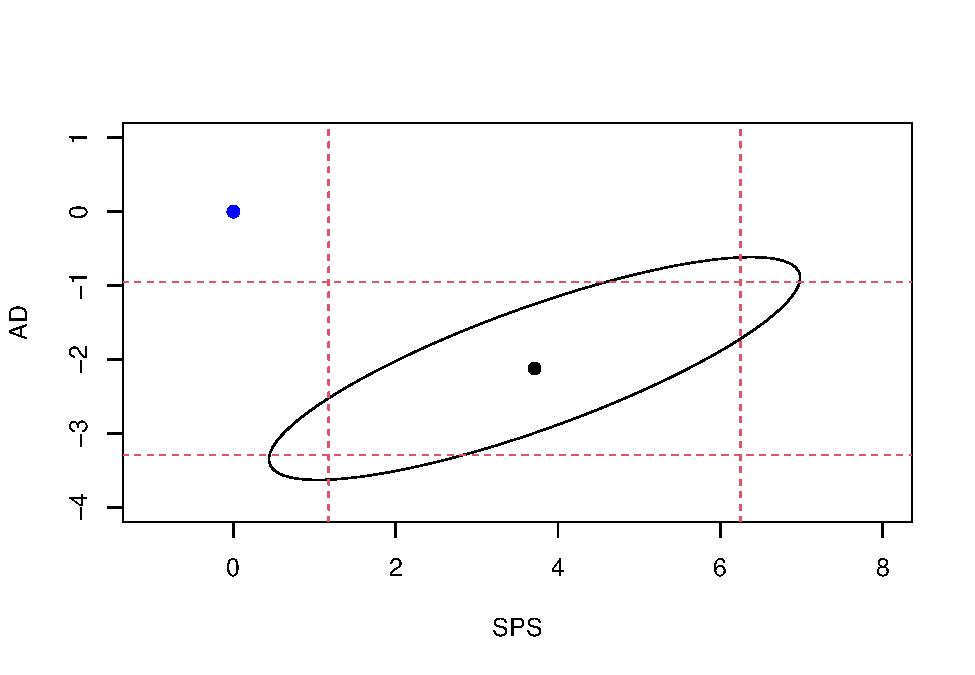
\includegraphics{code_files/figure-latex/unnamed-chunk-6-1.pdf}

El origen de coordenadas nos indica el resultado del test de Wald bajo
las siguientes hipótesis:

\begin{itemize}
\tightlist
\item
  H0: \(\beta1 = \beta2 = 0\). Los coeficientes de ambas variables son
  0.
\item
  H1: \(\beta1\neq0\) y/o \(\beta2\neq0\). Caso contrario, al menos uno
  de los coeficientes no es 0.
\end{itemize}

Si la elipse de confianza no incluye el (0,0), esto sugiere que los
coeficientes son distintos a 0 de forma estadísticamente significativa.
Esto sugiere que las variables predictoras usadas para construir la
elipse, tienen un efecto sobre la variable respuesta. Por otro lado, si
no se incluye, indica que los coeficientes estimados no son distintos
que 0 y que por lo tanto las variables predictoras no aportan al modelo.
Esto no es necesariamente cierto, ya que existen múltiples motivos por
los cuales la elipse incluiría el (0,0), como por ejemplo, que el modelo
no sea lineal, y por lo tanto no veamos relación.

En este caso al no incluirlo, podemos deducir que las variables SPS y AD
sí explican la variable BD.

\hypertarget{f-predicciuxf3n}{%
\subsubsection{(f) Predicción}\label{f-predicciuxf3n}}

\begin{Shaded}
\begin{Highlighting}[]
\NormalTok{new\_ob }\OtherTok{=} \FunctionTok{data.frame}\NormalTok{(}\AttributeTok{SPS =} \DecValTok{5}\NormalTok{, }\AttributeTok{AD =} \DecValTok{11}\NormalTok{)}
\CommentTok{\#install.packages(\textquotesingle{}regclass\textquotesingle{})}
\FunctionTok{library}\NormalTok{(regclass)}
\end{Highlighting}
\end{Shaded}

\begin{verbatim}
## Loading required package: bestglm
\end{verbatim}

\begin{verbatim}
## Loading required package: leaps
\end{verbatim}

\begin{verbatim}
## Loading required package: VGAM
\end{verbatim}

\begin{verbatim}
## Loading required package: stats4
\end{verbatim}

\begin{verbatim}
## Loading required package: splines
\end{verbatim}

\begin{verbatim}
## 
## Attaching package: 'VGAM'
\end{verbatim}

\begin{verbatim}
## The following object is masked from 'package:car':
## 
##     logit
\end{verbatim}

\begin{verbatim}
## Loading required package: rpart
\end{verbatim}

\begin{verbatim}
## Loading required package: randomForest
\end{verbatim}

\begin{verbatim}
## randomForest 4.7-1.1
\end{verbatim}

\begin{verbatim}
## Type rfNews() to see new features/changes/bug fixes.
\end{verbatim}

\begin{verbatim}
## Important regclass change from 1.3:
## All functions that had a . in the name now have an _
## all.correlations -> all_correlations, cor.demo -> cor_demo, etc.
\end{verbatim}

\begin{Shaded}
\begin{Highlighting}[]
\FunctionTok{extrapolation\_check}\NormalTok{(lmod\_red,new\_ob)}
\end{Highlighting}
\end{Shaded}

\begin{verbatim}
##   Observation Percentile
## 1           1         25
\end{verbatim}

\begin{Shaded}
\begin{Highlighting}[]
\CommentTok{\# Alternativamente}
\NormalTok{range\_SPS }\OtherTok{=} \FunctionTok{range}\NormalTok{(data1}\SpecialCharTok{$}\NormalTok{SPS)}
\NormalTok{range\_AD }\OtherTok{=} \FunctionTok{range}\NormalTok{(data1}\SpecialCharTok{$}\NormalTok{AD)}
\FunctionTok{cat}\NormalTok{(}\StringTok{"Min AD:"}\NormalTok{, range\_AD[}\DecValTok{1}\NormalTok{], }\StringTok{" Max AD:"}\NormalTok{, range\_AD[}\DecValTok{2}\NormalTok{], }\StringTok{" Observed value:"}\NormalTok{, new\_ob}\SpecialCharTok{$}\NormalTok{AD)}
\end{Highlighting}
\end{Shaded}

\begin{verbatim}
## Min AD: 5  Max AD: 19  Observed value: 11
\end{verbatim}

\begin{Shaded}
\begin{Highlighting}[]
\FunctionTok{cat}\NormalTok{(}\StringTok{"}\SpecialCharTok{\textbackslash{}n}\StringTok{"}\NormalTok{)}
\end{Highlighting}
\end{Shaded}

\begin{Shaded}
\begin{Highlighting}[]
\FunctionTok{cat}\NormalTok{(}\StringTok{"Min SPS:"}\NormalTok{, range\_SPS[}\DecValTok{1}\NormalTok{], }\StringTok{" Max SPS:"}\NormalTok{, range\_SPS[}\DecValTok{2}\NormalTok{], }\StringTok{" Observed value:"}\NormalTok{, new\_ob}\SpecialCharTok{$}\NormalTok{SPS)}
\end{Highlighting}
\end{Shaded}

\begin{verbatim}
## Min SPS: 1  Max SPS: 7  Observed value: 5
\end{verbatim}

\begin{Shaded}
\begin{Highlighting}[]
\CommentTok{\# create a scatter plot of SPS and AD}
\FunctionTok{plot}\NormalTok{(SPS }\SpecialCharTok{\textasciitilde{}}\NormalTok{ AD, }\AttributeTok{data =}\NormalTok{ data1)}

\CommentTok{\# add the observed values as points on the plot}
\FunctionTok{points}\NormalTok{(}\AttributeTok{x =} \DecValTok{11}\NormalTok{, }\AttributeTok{y =} \DecValTok{5}\NormalTok{, }\AttributeTok{col =} \StringTok{"red"}\NormalTok{, }\AttributeTok{pch =} \DecValTok{19}\NormalTok{)}

\CommentTok{\# add a legend to the plot}
\FunctionTok{legend}\NormalTok{(}\StringTok{"topright"}\NormalTok{, }\AttributeTok{legend =} \FunctionTok{c}\NormalTok{(}\StringTok{"Observed values"}\NormalTok{), }\AttributeTok{col =} \FunctionTok{c}\NormalTok{(}\StringTok{"red"}\NormalTok{), }\AttributeTok{pch =} \DecValTok{19}\NormalTok{)}
\end{Highlighting}
\end{Shaded}

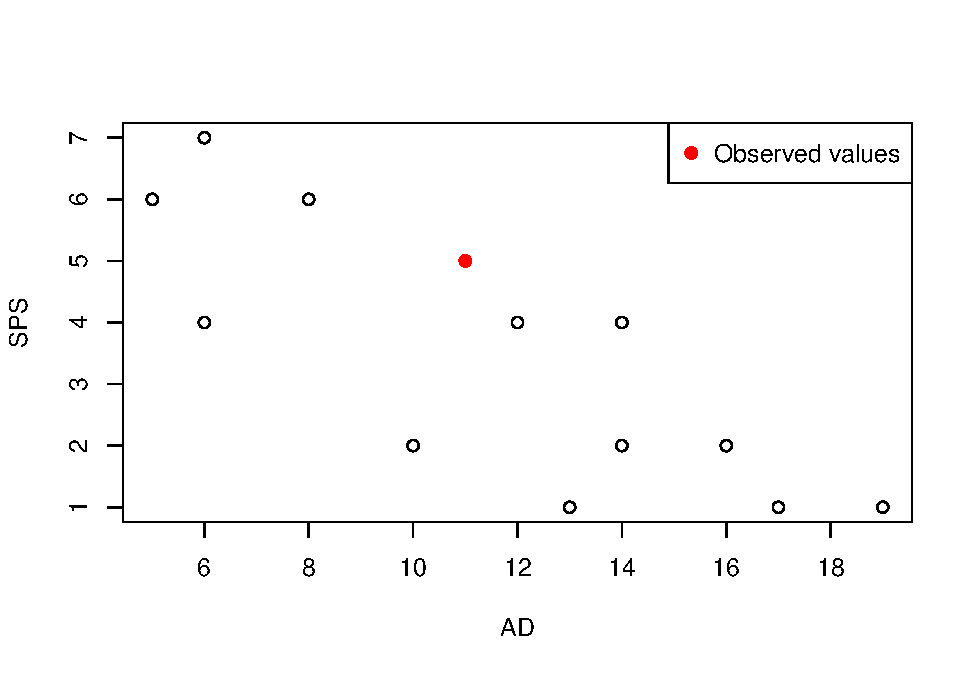
\includegraphics{code_files/figure-latex/unnamed-chunk-8-1.pdf}

En este paquete (regclass) percentiles de aproximadamente 99 pueden
implicar extrapolación, en nuestro caso obtenemos un percentil de 25
indicando que seguramente no la haya. Si revisamos el scatterplot
podemos ver que estos valores de SPS y AD entran dentro del scope del
modelo. Usando la función range también podemos determinarlo, ya que nos
indica el mínimo y el máximo de las variables señaladas. Si nuestra
observación cae en ese rango no es una extrapolación.

\begin{Shaded}
\begin{Highlighting}[]
\NormalTok{pred }\OtherTok{\textless{}{-}} \FunctionTok{predict}\NormalTok{(lmod\_red, new\_ob, }\AttributeTok{interval =} \StringTok{"confidence"}\NormalTok{, }\AttributeTok{level =} \FloatTok{0.95}\NormalTok{)}
\FunctionTok{cat}\NormalTok{(}\StringTok{"Predicted value:"}\NormalTok{, pred[}\DecValTok{1}\NormalTok{], }\StringTok{"}\SpecialCharTok{\textbackslash{}n}\StringTok{"}\NormalTok{)}
\end{Highlighting}
\end{Shaded}

\begin{verbatim}
## Predicted value: 30.76569
\end{verbatim}

\begin{Shaded}
\begin{Highlighting}[]
\FunctionTok{cat}\NormalTok{(}\StringTok{"95\% confidence interval:"}\NormalTok{, pred[}\DecValTok{2}\NormalTok{], }\StringTok{"{-}"}\NormalTok{, pred[}\DecValTok{3}\NormalTok{])}
\end{Highlighting}
\end{Shaded}

\begin{verbatim}
## 95% confidence interval: 26.05199 - 35.47939
\end{verbatim}

\hypertarget{ejercicio-2}{%
\section{Ejercicio 2}\label{ejercicio-2}}

\hypertarget{a-gruxe1fico-de-dispersiuxf3n}{%
\subsubsection{(a) Gráfico de
dispersión}\label{a-gruxe1fico-de-dispersiuxf3n}}

\begin{Shaded}
\begin{Highlighting}[]
\CommentTok{\#install.packages("readxl")}
\FunctionTok{library}\NormalTok{(}\StringTok{"readxl"}\NormalTok{)}
\NormalTok{data2 }\OtherTok{=} \FunctionTok{read.csv}\NormalTok{(}\StringTok{"lions.csv"}\NormalTok{)}
\end{Highlighting}
\end{Shaded}

\begin{Shaded}
\begin{Highlighting}[]
\FunctionTok{library}\NormalTok{(ggplot2)}
\end{Highlighting}
\end{Shaded}

\begin{verbatim}
## 
## Attaching package: 'ggplot2'
\end{verbatim}

\begin{verbatim}
## The following object is masked from 'package:randomForest':
## 
##     margin
\end{verbatim}

\begin{Shaded}
\begin{Highlighting}[]
\FunctionTok{library}\NormalTok{(dplyr)}
\end{Highlighting}
\end{Shaded}

\begin{verbatim}
## 
## Attaching package: 'dplyr'
\end{verbatim}

\begin{verbatim}
## The following object is masked from 'package:randomForest':
## 
##     combine
\end{verbatim}

\begin{verbatim}
## The following object is masked from 'package:car':
## 
##     recode
\end{verbatim}

\begin{verbatim}
## The following objects are masked from 'package:stats':
## 
##     filter, lag
\end{verbatim}

\begin{verbatim}
## The following objects are masked from 'package:base':
## 
##     intersect, setdiff, setequal, union
\end{verbatim}

\begin{Shaded}
\begin{Highlighting}[]
\NormalTok{p }\OtherTok{=} \FunctionTok{ggplot}\NormalTok{(data2, }\FunctionTok{aes}\NormalTok{(age, prop.black))}
\NormalTok{p }\SpecialCharTok{+} \FunctionTok{geom\_point}\NormalTok{(}\FunctionTok{aes}\NormalTok{(}\AttributeTok{shape =} \FunctionTok{paste}\NormalTok{(}\FunctionTok{ifelse}\NormalTok{(sex }\SpecialCharTok{==} \StringTok{"M"}\NormalTok{, }\StringTok{"males"}\NormalTok{, }\StringTok{"females"}\NormalTok{), }\FunctionTok{ifelse}\NormalTok{(area }\SpecialCharTok{==} \StringTok{"N"}\NormalTok{, }\StringTok{"Ngorongoro"}\NormalTok{, }\StringTok{"Serengeti"}\NormalTok{)))) }\SpecialCharTok{+} 
  \FunctionTok{scale\_shape\_manual}\NormalTok{(}\AttributeTok{name =} \StringTok{""}\NormalTok{, }
                     \AttributeTok{values =} \FunctionTok{c}\NormalTok{(}\DecValTok{1}\NormalTok{, }\DecValTok{19}\NormalTok{, }\DecValTok{2}\NormalTok{, }\DecValTok{17}\NormalTok{), }
                     \AttributeTok{labels =}\NormalTok{ data2 }\SpecialCharTok{\%\textgreater{}\%}
                       \FunctionTok{group\_by}\NormalTok{(sex, area) }\SpecialCharTok{\%\textgreater{}\%}
                       \FunctionTok{summarize}\NormalTok{(}\AttributeTok{n =} \FunctionTok{n}\NormalTok{()) }\SpecialCharTok{\%\textgreater{}\%}
                       \FunctionTok{mutate}\NormalTok{(}\AttributeTok{label =} \FunctionTok{paste0}\NormalTok{(}\FunctionTok{ifelse}\NormalTok{(area }\SpecialCharTok{==} \StringTok{"N"}\NormalTok{, }\StringTok{"Ngorongoro"}\NormalTok{, }\StringTok{"Serengeti"}\NormalTok{), }\StringTok{" "}\NormalTok{, }\FunctionTok{ifelse}\NormalTok{(sex }\SpecialCharTok{==} \StringTok{"M"}\NormalTok{, }\StringTok{"males"}\NormalTok{, }\StringTok{"females"}\NormalTok{), }\StringTok{"(n = "}\NormalTok{, n, }\StringTok{")"}\NormalTok{)) }\SpecialCharTok{\%\textgreater{}\%}
                       \FunctionTok{pull}\NormalTok{(label)) }\SpecialCharTok{+}
  \FunctionTok{labs}\NormalTok{(}\AttributeTok{x =} \StringTok{"Age (yr)"}\NormalTok{, }\AttributeTok{y =} \StringTok{"Proportion black"}\NormalTok{, }\AttributeTok{shape =} \StringTok{""}\NormalTok{) }\SpecialCharTok{+}
  \FunctionTok{scale\_x\_continuous}\NormalTok{(}\AttributeTok{breaks =} \FunctionTok{seq}\NormalTok{(}\DecValTok{0}\NormalTok{, }\DecValTok{16}\NormalTok{, }\DecValTok{2}\NormalTok{), }\AttributeTok{limits =} \FunctionTok{c}\NormalTok{(}\DecValTok{0}\NormalTok{, }\DecValTok{16}\NormalTok{)) }\SpecialCharTok{+}
  \FunctionTok{scale\_y\_continuous}\NormalTok{(}\AttributeTok{breaks =} \FunctionTok{seq}\NormalTok{(}\DecValTok{0}\NormalTok{, }\DecValTok{1}\NormalTok{, }\FloatTok{0.2}\NormalTok{), }\AttributeTok{limits =} \FunctionTok{c}\NormalTok{(}\DecValTok{0}\NormalTok{, }\DecValTok{1}\NormalTok{)) }\SpecialCharTok{+}
  \FunctionTok{scale\_fill\_discrete}\NormalTok{(}\AttributeTok{breaks=}\FunctionTok{c}\NormalTok{(}\StringTok{\textquotesingle{}F\textquotesingle{}}\NormalTok{, }\StringTok{\textquotesingle{}M\textquotesingle{}}\NormalTok{)) }\SpecialCharTok{+}
  \FunctionTok{theme\_classic}\NormalTok{() }\SpecialCharTok{+}
  \FunctionTok{theme}\NormalTok{(}\AttributeTok{aspect.ratio =} \FloatTok{0.5}\NormalTok{, }\AttributeTok{legend.position =} \FunctionTok{c}\NormalTok{(}\FloatTok{0.75}\NormalTok{, }\FloatTok{0.3}\NormalTok{))}
\end{Highlighting}
\end{Shaded}

\begin{verbatim}
## `summarise()` has grouped output by 'sex'. You can override using the `.groups`
## argument.
\end{verbatim}

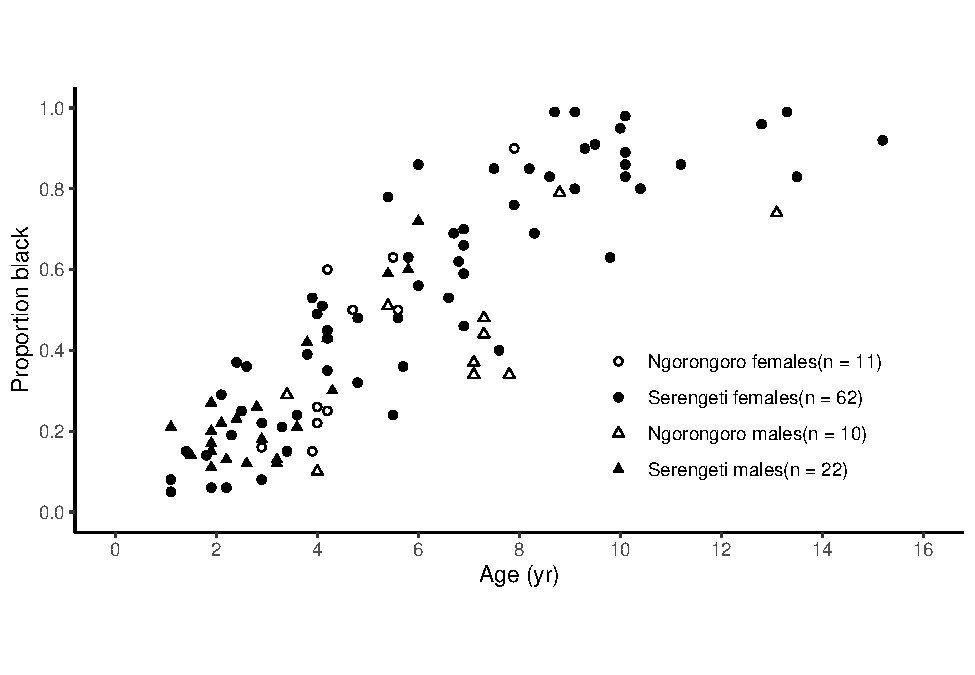
\includegraphics{code_files/figure-latex/unnamed-chunk-11-1.pdf}

\hypertarget{b-modelos-seguxfan-uxe1rea}{%
\subsubsection{(b) Modelos según
área}\label{b-modelos-seguxfan-uxe1rea}}

\begin{Shaded}
\begin{Highlighting}[]
\NormalTok{lmod\_all }\OtherTok{=} \FunctionTok{lm}\NormalTok{(prop.black }\SpecialCharTok{\textasciitilde{}}\NormalTok{ age }\SpecialCharTok{*}\NormalTok{ (sex }\SpecialCharTok{+}\NormalTok{ area), }\AttributeTok{data =}\NormalTok{ data2)}
\FunctionTok{summary}\NormalTok{(lmod\_all)}
\end{Highlighting}
\end{Shaded}

\begin{verbatim}
## 
## Call:
## lm(formula = prop.black ~ age * (sex + area), data = data2)
## 
## Residuals:
##      Min       1Q   Median       3Q      Max 
## -0.32206 -0.09746 -0.01365  0.10173  0.32558 
## 
## Coefficients:
##              Estimate Std. Error t value Pr(>|t|)    
## (Intercept)  0.003101   0.105559   0.029 0.976627    
## age          0.081609   0.021302   3.831 0.000224 ***
## sexM        -0.005786   0.071180  -0.081 0.935374    
## areaS        0.069820   0.106242   0.657 0.512593    
## age:sexM    -0.015094   0.017246  -0.875 0.383571    
## age:areaS   -0.004692   0.021184  -0.221 0.825161    
## ---
## Signif. codes:  0 '***' 0.001 '**' 0.01 '*' 0.05 '.' 0.1 ' ' 1
## 
## Residual standard error: 0.1373 on 99 degrees of freedom
## Multiple R-squared:  0.7738, Adjusted R-squared:  0.7624 
## F-statistic: 67.74 on 5 and 99 DF,  p-value: < 2.2e-16
\end{verbatim}

\begin{Shaded}
\begin{Highlighting}[]
\NormalTok{data2\_split\_area }\OtherTok{=} \FunctionTok{split}\NormalTok{(data2, }\AttributeTok{f=}\NormalTok{data2}\SpecialCharTok{$}\NormalTok{area)}

\NormalTok{lmod\_N }\OtherTok{=} \FunctionTok{lm}\NormalTok{(prop.black }\SpecialCharTok{\textasciitilde{}}\NormalTok{ age }\SpecialCharTok{*}\NormalTok{ sex, }\AttributeTok{data =}\NormalTok{ data2\_split\_area}\SpecialCharTok{$}\NormalTok{N)}
\NormalTok{lmod\_S }\OtherTok{=} \FunctionTok{lm}\NormalTok{(prop.black }\SpecialCharTok{\textasciitilde{}}\NormalTok{ age }\SpecialCharTok{*}\NormalTok{ sex, }\AttributeTok{data =}\NormalTok{ data2\_split\_area}\SpecialCharTok{$}\NormalTok{S)}
\FunctionTok{summary}\NormalTok{(lmod\_N)}
\end{Highlighting}
\end{Shaded}

\begin{verbatim}
## 
## Call:
## lm(formula = prop.black ~ age * sex, data = data2_split_area$N)
## 
## Residuals:
##      Min       1Q   Median       3Q      Max 
## -0.15771 -0.08862 -0.02669  0.06724  0.25969 
## 
## Coefficients:
##             Estimate Std. Error t value Pr(>|t|)    
## (Intercept) -0.32531    0.14975  -2.172   0.0443 *  
## age          0.15848    0.03112   5.092 9.04e-05 ***
## sexM         0.35005    0.19249   1.819   0.0866 .  
## age:sexM    -0.10024    0.03498  -2.866   0.0107 *  
## ---
## Signif. codes:  0 '***' 0.001 '**' 0.01 '*' 0.05 '.' 0.1 ' ' 1
## 
## Residual standard error: 0.1293 on 17 degrees of freedom
## Multiple R-squared:  0.6991, Adjusted R-squared:  0.6461 
## F-statistic: 13.17 on 3 and 17 DF,  p-value: 0.000108
\end{verbatim}

\begin{Shaded}
\begin{Highlighting}[]
\FunctionTok{summary}\NormalTok{(lmod\_S)}
\end{Highlighting}
\end{Shaded}

\begin{verbatim}
## 
## Call:
## lm(formula = prop.black ~ age * sex, data = data2_split_area$S)
## 
## Residuals:
##      Min       1Q   Median       3Q      Max 
## -0.30712 -0.08717  0.02071  0.09153  0.33028 
## 
## Coefficients:
##              Estimate Std. Error t value Pr(>|t|)    
## (Intercept)  0.074893   0.035288   2.122   0.0369 *  
## age          0.075804   0.004905  15.454   <2e-16 ***
## sexM        -0.130055   0.076583  -1.698   0.0934 .  
## age:sexM     0.031156   0.021058   1.480   0.1429    
## ---
## Signif. codes:  0 '***' 0.001 '**' 0.01 '*' 0.05 '.' 0.1 ' ' 1
## 
## Residual standard error: 0.1307 on 80 degrees of freedom
## Multiple R-squared:  0.8116, Adjusted R-squared:  0.8046 
## F-statistic: 114.9 on 3 and 80 DF,  p-value: < 2.2e-16
\end{verbatim}

En el modelo con todas las variable, podemos observar que el sexo no
influye significativamente sobre la variable respuesta (proporción de
negro en la nariz), con un pvalor = 0.93.

Al separar por área, seguimos obteniendo que el sexo no influye de forma
significativa para ninguna de las dos áreas, al menos para un nivel de
significación del 0.05. Si tomamos un nivel de 0.1, entonces en ambos el
sexo pasa a ser significativo. En la población Ngorongoro los machos
tienen la nariz más oscura que las hembras (coef sexM = 0.35), mientras
que en los Serengeti los machos tienen la nariz más clara (coef sexM =
-0.13).

Es importante estudiar la interacción entre la edad y el sexo. En el
caso de los Serengeti ésta no es significativa. Y por lo tanto, los
resultados se alinean con los del artículo (no hay efecto del sexo en el
color de la nariz de los leones Serengeti). En cambio, en el caso de los
Ngorongoro sí lo es (pv = 0.01), esto quiere decir que según la edad de
los leones, sí observamos diferencias en cuanto al sexo y el color de la
nariz. Nuevamente los hallazgos coindicen con los del artículo, pues los
machos Ngorongoro tienen narices más claras que las hembras a ciertas
edades (coef age:sexM = -0.1)

\hypertarget{c-modelo-leones-macho}{%
\subsubsection{(c) Modelo leones macho}\label{c-modelo-leones-macho}}

\begin{Shaded}
\begin{Highlighting}[]
\NormalTok{data2\_split\_sex }\OtherTok{=} \FunctionTok{split}\NormalTok{(data2, }\AttributeTok{f =}\NormalTok{ data2}\SpecialCharTok{$}\NormalTok{sex)}
\NormalTok{lmod\_male }\OtherTok{=} \FunctionTok{lm}\NormalTok{(prop.black }\SpecialCharTok{\textasciitilde{}}\NormalTok{ age }\SpecialCharTok{*}\NormalTok{ area, }\AttributeTok{data =}\NormalTok{ data2\_split\_sex}\SpecialCharTok{$}\NormalTok{M)}
\FunctionTok{summary}\NormalTok{(lmod\_male)}
\end{Highlighting}
\end{Shaded}

\begin{verbatim}
## 
## Call:
## lm(formula = prop.black ~ age * area, data = data2_split_sex$M)
## 
## Residuals:
##      Min       1Q   Median       3Q      Max 
## -0.16711 -0.08083  0.01880  0.05576  0.25274 
## 
## Coefficients:
##             Estimate Std. Error t value Pr(>|t|)    
## (Intercept)  0.02474    0.10178   0.243  0.80971    
## age          0.05824    0.01343   4.335  0.00017 ***
## areaS       -0.07990    0.11646  -0.686  0.49831    
## age:areaS    0.04872    0.02171   2.244  0.03292 *  
## ---
## Signif. codes:  0 '***' 0.001 '**' 0.01 '*' 0.05 '.' 0.1 ' ' 1
## 
## Residual standard error: 0.1088 on 28 degrees of freedom
## Multiple R-squared:  0.7286, Adjusted R-squared:  0.6995 
## F-statistic: 25.05 on 3 and 28 DF,  p-value: 4.408e-08
\end{verbatim}

Para los machos, no existen diferencias significativas según el área (pv
= 0.49). Similarmente al apartado anterior, sí existe significación en
la interacción de la edad y el área (pv = 0.03). Esto quiere decir, que
según la edad del león sí encontraremos diferencias por área. En
específico, los machos Serengeti tienen la nariz más oscura que los
Ngorongoro (coef age:areaS = 0.04). Podemos ver este efecto más
claramente en el siguiente gráfico. Para un león de 2 años no existen
diferencias según el área, pero para un león de 8 años sí lo hay, siendo
más oscura la de los Serengeti (mayor proporción de negro).

\begin{Shaded}
\begin{Highlighting}[]
\CommentTok{\# Create a sequence of ages to use for plotting}
\NormalTok{age\_seq }\OtherTok{\textless{}{-}} \FunctionTok{seq}\NormalTok{(}\FunctionTok{min}\NormalTok{(data2\_split\_sex}\SpecialCharTok{$}\NormalTok{M}\SpecialCharTok{$}\NormalTok{age), }\FunctionTok{max}\NormalTok{(data2\_split\_sex}\SpecialCharTok{$}\NormalTok{M}\SpecialCharTok{$}\NormalTok{age), }\AttributeTok{length.out =} \DecValTok{100}\NormalTok{)}

\CommentTok{\# Predict proportion black for each area at each age}
\NormalTok{pred\_N }\OtherTok{\textless{}{-}} \FunctionTok{predict}\NormalTok{(lmod\_male, }\AttributeTok{newdata =} \FunctionTok{data.frame}\NormalTok{(}\AttributeTok{age =}\NormalTok{ age\_seq, }\AttributeTok{area =} \StringTok{"N"}\NormalTok{))}
\NormalTok{pred\_S }\OtherTok{\textless{}{-}} \FunctionTok{predict}\NormalTok{(lmod\_male, }\AttributeTok{newdata =} \FunctionTok{data.frame}\NormalTok{(}\AttributeTok{age =}\NormalTok{ age\_seq, }\AttributeTok{area =} \StringTok{"S"}\NormalTok{))}

\CommentTok{\# Plot regression lines for each area}
\FunctionTok{plot}\NormalTok{(data2\_split\_sex}\SpecialCharTok{$}\NormalTok{M}\SpecialCharTok{$}\NormalTok{age, data2\_split\_sex}\SpecialCharTok{$}\NormalTok{M}\SpecialCharTok{$}\NormalTok{prop.black, }\AttributeTok{xlab =} \StringTok{"Age"}\NormalTok{, }\AttributeTok{ylab =} \StringTok{"Proportion Black"}\NormalTok{)}
\FunctionTok{lines}\NormalTok{(age\_seq, pred\_N, }\AttributeTok{col =} \StringTok{"red"}\NormalTok{)}
\FunctionTok{lines}\NormalTok{(age\_seq, pred\_S, }\AttributeTok{col =} \StringTok{"blue"}\NormalTok{)}
\FunctionTok{legend}\NormalTok{(}\StringTok{"bottomright"}\NormalTok{, }\AttributeTok{legend =} \FunctionTok{c}\NormalTok{(}\StringTok{"Ngorongoro"}\NormalTok{, }\StringTok{"Serengeti"}\NormalTok{), }\AttributeTok{col =} \FunctionTok{c}\NormalTok{(}\StringTok{"red"}\NormalTok{, }\StringTok{"blue"}\NormalTok{), }\AttributeTok{lty =} \DecValTok{1}\NormalTok{)}
\end{Highlighting}
\end{Shaded}

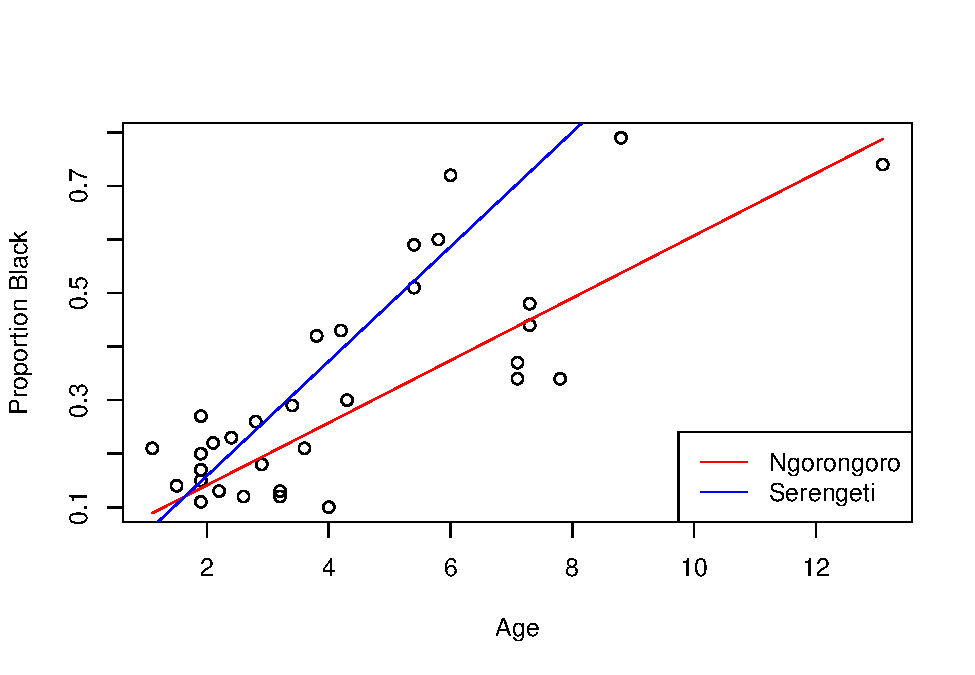
\includegraphics{code_files/figure-latex/unnamed-chunk-14-1.pdf}

\hypertarget{d-predicciuxf3n-de-la-edad-de-una-leona}{%
\subsubsection{(d) Predicción de la edad de una
leona}\label{d-predicciuxf3n-de-la-edad-de-una-leona}}

No, ninguno de los modelos ajustados hasta el momento serviría para
predecir la edad de una leona según su proporción de pigmentación. Hasta
ahora hemos usado la pigmentación de la nariz como variable respuesta,
que era explicada por la edad, área y sexo del león. No es posible
simplemente ``revertir'' el modelo, necesitaríamos estimar un nuevo
modelo dónde la variable respuesta fuera la edad, y la variable
predictora fuera el color de la nariz.

El modelo que proponen en el artículo, utilizan la función arcsin(sqrt)
para transformar la proporción de negro en la nariz, y hacerla más
simétrica y adecuada para el estudio estadístico.

\begin{Shaded}
\begin{Highlighting}[]
\FunctionTok{library}\NormalTok{(stats)}

\CommentTok{\# Aplicamos la transformación sólo a }
\NormalTok{data2\_split\_sex}\SpecialCharTok{$}\NormalTok{F}\SpecialCharTok{$}\NormalTok{prop.black.transformed }\OtherTok{=} \FunctionTok{asin}\NormalTok{(}\FunctionTok{sqrt}\NormalTok{(data2\_split\_sex}\SpecialCharTok{$}\NormalTok{F}\SpecialCharTok{$}\NormalTok{prop.black))}

\NormalTok{lmod\_age }\OtherTok{=} \FunctionTok{lm}\NormalTok{(age }\SpecialCharTok{\textasciitilde{}}\NormalTok{ prop.black.transformed, }\AttributeTok{data =}\NormalTok{ data2\_split\_sex}\SpecialCharTok{$}\NormalTok{F)}

\CommentTok{\# Compute the predicted age on the transformed scale}

\CommentTok{\# Define the proportion black for which to make the prediction}
\NormalTok{prop\_black }\OtherTok{=} \FloatTok{0.5}
\NormalTok{prop\_black\_transformed }\OtherTok{\textless{}{-}} \FunctionTok{asin}\NormalTok{(}\FunctionTok{sqrt}\NormalTok{(prop\_black))}

\CommentTok{\# Compute the predicted age and confidence intervals}
\NormalTok{predicted\_age }\OtherTok{\textless{}{-}} \FunctionTok{predict}\NormalTok{(lmod\_age, }\AttributeTok{newdata =} \FunctionTok{data.frame}\NormalTok{(}\AttributeTok{prop.black.transformed =}\NormalTok{ prop\_black\_transformed))}
\NormalTok{ci\_95 }\OtherTok{\textless{}{-}} \FunctionTok{predict}\NormalTok{(lmod\_age, }\AttributeTok{newdata =} \FunctionTok{data.frame}\NormalTok{(}\AttributeTok{prop.black.transformed =}\NormalTok{ prop\_black\_transformed), }\AttributeTok{interval =} \StringTok{"prediction"}\NormalTok{, }\AttributeTok{level =} \FloatTok{0.95}\NormalTok{)}
\NormalTok{ci\_75 }\OtherTok{\textless{}{-}} \FunctionTok{predict}\NormalTok{(lmod\_age, }\AttributeTok{newdata =} \FunctionTok{data.frame}\NormalTok{(}\AttributeTok{prop.black.transformed =}\NormalTok{ prop\_black\_transformed), }\AttributeTok{interval =} \StringTok{"prediction"}\NormalTok{, }\AttributeTok{level =} \FloatTok{0.75}\NormalTok{)}
\NormalTok{ci\_50 }\OtherTok{\textless{}{-}} \FunctionTok{predict}\NormalTok{(lmod\_age, }\AttributeTok{newdata =} \FunctionTok{data.frame}\NormalTok{(}\AttributeTok{prop.black.transformed =}\NormalTok{ prop\_black\_transformed), }\AttributeTok{interval =} \StringTok{"prediction"}\NormalTok{, }\AttributeTok{level =} \FloatTok{0.50}\NormalTok{)}

\CommentTok{\# Compute se}
\NormalTok{summary\_lmod\_age }\OtherTok{\textless{}{-}} \FunctionTok{summary}\NormalTok{(lmod\_age)}
\NormalTok{se\_predicted\_age }\OtherTok{\textless{}{-}}\NormalTok{ summary\_lmod\_age}\SpecialCharTok{$}\NormalTok{sigma }\SpecialCharTok{*} \FunctionTok{sqrt}\NormalTok{(}\DecValTok{1} \SpecialCharTok{+} \DecValTok{1}\SpecialCharTok{/}\FunctionTok{nrow}\NormalTok{(data2\_split\_sex}\SpecialCharTok{$}\NormalTok{F) }\SpecialCharTok{+}\NormalTok{ (prop\_black\_transformed }\SpecialCharTok{{-}} \FunctionTok{mean}\NormalTok{(data2\_split\_sex}\SpecialCharTok{$}\NormalTok{F}\SpecialCharTok{$}\NormalTok{prop.black.transformed))}\SpecialCharTok{\^{}}\DecValTok{2}\SpecialCharTok{/}\FunctionTok{var}\NormalTok{(data2\_split\_sex}\SpecialCharTok{$}\NormalTok{F}\SpecialCharTok{$}\NormalTok{prop.black.transformed))}

\CommentTok{\# Create a data frame with the predicted age and confidence intervals}
\NormalTok{result\_table }\OtherTok{\textless{}{-}} \FunctionTok{data.frame}\NormalTok{(}\StringTok{"Proportion black"} \OtherTok{=}\NormalTok{ prop\_black, }
                           \StringTok{"Estimated age in years"} \OtherTok{=}\FunctionTok{paste}\NormalTok{(}\FunctionTok{round}\NormalTok{(predicted\_age,}\DecValTok{2}\NormalTok{), }\StringTok{"("}\NormalTok{, }\FunctionTok{round}\NormalTok{(se\_predicted\_age,}\DecValTok{2}\NormalTok{), }\StringTok{")"}\NormalTok{),}
                           \StringTok{"95\% CI"} \OtherTok{=} \FunctionTok{paste}\NormalTok{(}\FunctionTok{round}\NormalTok{(ci\_95[}\DecValTok{2}\NormalTok{],}\DecValTok{2}\NormalTok{), }\FunctionTok{round}\NormalTok{(ci\_95[}\DecValTok{3}\NormalTok{],}\DecValTok{2}\NormalTok{), }\AttributeTok{sep =} \StringTok{"{-}"}\NormalTok{),}
                           \StringTok{"75\% CI"} \OtherTok{=} \FunctionTok{paste}\NormalTok{(}\FunctionTok{round}\NormalTok{(ci\_75[}\DecValTok{2}\NormalTok{],}\DecValTok{2}\NormalTok{), }\FunctionTok{round}\NormalTok{(ci\_75[}\DecValTok{3}\NormalTok{],}\DecValTok{2}\NormalTok{), }\AttributeTok{sep =} \StringTok{"{-}"}\NormalTok{),}
                           \StringTok{"50\% CI"} \OtherTok{=} \FunctionTok{paste}\NormalTok{(}\FunctionTok{round}\NormalTok{(ci\_50[}\DecValTok{2}\NormalTok{],}\DecValTok{2}\NormalTok{), }\FunctionTok{round}\NormalTok{(ci\_50[}\DecValTok{3}\NormalTok{],}\DecValTok{2}\NormalTok{), }\AttributeTok{sep =} \StringTok{"{-}"}\NormalTok{))}

\FunctionTok{library}\NormalTok{(knitr)}

\NormalTok{new\_names }\OtherTok{=} \FunctionTok{c}\NormalTok{(}\StringTok{"Proportion black"}\NormalTok{, }\StringTok{"Estimated age in years (s.e.)"}\NormalTok{, }\StringTok{"95\% p.i."}\NormalTok{, }\StringTok{"75\% p.i."}\NormalTok{, }\StringTok{"50\% p.i."}\NormalTok{)}

\FunctionTok{names}\NormalTok{(result\_table) }\OtherTok{\textless{}{-}}\NormalTok{ new\_names}

\CommentTok{\# Create a table using the kable function from the knitr package}
\FunctionTok{kable}\NormalTok{(result\_table, }\AttributeTok{format =} \StringTok{"markdown"}\NormalTok{)}
\end{Highlighting}
\end{Shaded}

\begin{longtable}[]{@{}
  >{\raggedleft\arraybackslash}p{(\columnwidth - 8\tabcolsep) * \real{0.2267}}
  >{\raggedright\arraybackslash}p{(\columnwidth - 8\tabcolsep) * \real{0.4000}}
  >{\raggedright\arraybackslash}p{(\columnwidth - 8\tabcolsep) * \real{0.1200}}
  >{\raggedright\arraybackslash}p{(\columnwidth - 8\tabcolsep) * \real{0.1333}}
  >{\raggedright\arraybackslash}p{(\columnwidth - 8\tabcolsep) * \real{0.1200}}@{}}
\toprule()
\begin{minipage}[b]{\linewidth}\raggedleft
Proportion black
\end{minipage} & \begin{minipage}[b]{\linewidth}\raggedright
Estimated age in years (s.e.)
\end{minipage} & \begin{minipage}[b]{\linewidth}\raggedright
95\% p.i.
\end{minipage} & \begin{minipage}[b]{\linewidth}\raggedright
75\% p.i.
\end{minipage} & \begin{minipage}[b]{\linewidth}\raggedright
50\% p.i.
\end{minipage} \\
\midrule()
\endhead
0.5 & 5.71 ( 1.62 ) & 2.5-8.91 & 3.84-7.57 & 4.61-6.8 \\
\bottomrule()
\end{longtable}

Se o standard error es una medida de la variabilidad de los errores de
predicción de la variable dependiente a partir de las variables
independientes. Se calcula como la desviación estándar de los residuos
de la regresión (diferencias entre los valores predichos y los valores
observados) dividida por la raíz cuadrada del número de observaciones.En
resumen, el error estándar indica la precisión de las predicciones de la
variable dependiente y es una medida importante para evaluar la calidad
de un modelo de regresión lineal. Un error estándar más bajo indica una
mayor precisión en las predicciones del modelo.

\hypertarget{ejercicio-3}{%
\section{Ejercicio 3}\label{ejercicio-3}}

\hypertarget{a-gauss-markov-y-condiciones-del-modelo-re-regresiuxf3n}{%
\subsubsection{(a) Gauss-Markov y condiciones del modelo re
regresión}\label{a-gauss-markov-y-condiciones-del-modelo-re-regresiuxf3n}}

Las hipótesis de Gauss-Markov son:

\begin{itemize}
\tightlist
\item
  Linealidad: La relación entre la variable dependiente y las
  independientes debe ser lineal.
\item
  Independencia de errores
\item
  Homocedasticidad: La variancia de los errores o residuos debe ser
  constante entre todas las variables.
\item
  Normalidad de errores
\item
  No correlación de las variables independientes
\item
  Media condicional de 0: El valor esperado de los errores debe ser 0
  para todas las variables independientes
\end{itemize}

\hypertarget{linealidad}{%
\paragraph{Linealidad}\label{linealidad}}

\begin{Shaded}
\begin{Highlighting}[]
\CommentTok{\# Load required packages}
\FunctionTok{library}\NormalTok{(ggplot2)}

\CommentTok{\# Residuals vs. Fitted plot}
\FunctionTok{plot}\NormalTok{(lmod\_all, }\AttributeTok{which =} \DecValTok{1}\NormalTok{)}
\end{Highlighting}
\end{Shaded}

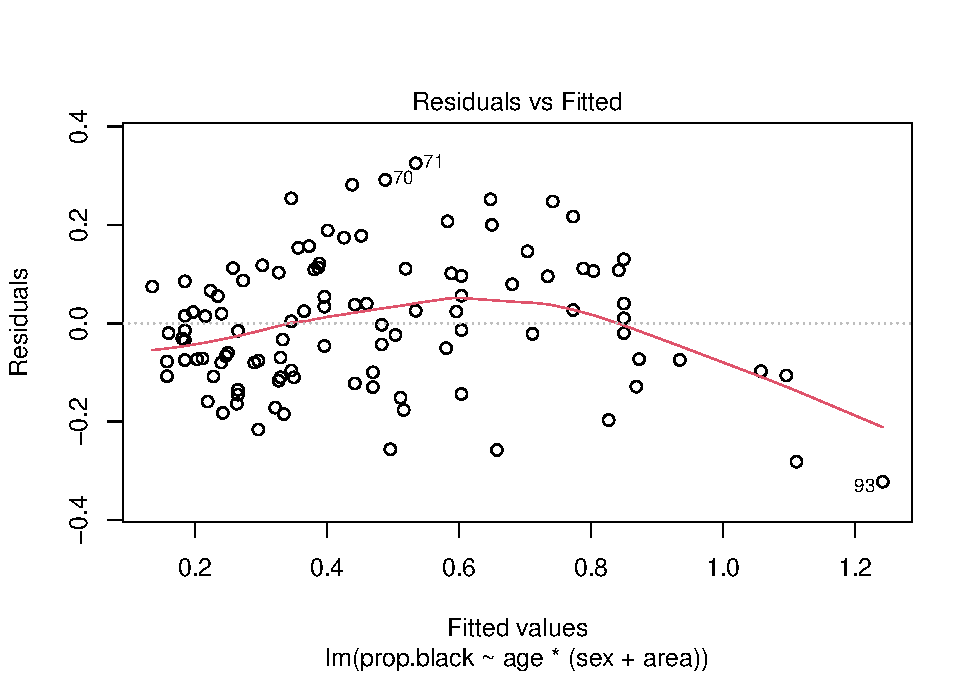
\includegraphics{code_files/figure-latex/unnamed-chunk-16-1.pdf}

\begin{Shaded}
\begin{Highlighting}[]
\CommentTok{\# Create dummy variables for sex and area}
\NormalTok{dummy\_sex }\OtherTok{\textless{}{-}} \FunctionTok{model.matrix}\NormalTok{(}\SpecialCharTok{\textasciitilde{}}\NormalTok{ sex, }\AttributeTok{data =}\NormalTok{ data2)}
\NormalTok{dummy\_area }\OtherTok{\textless{}{-}} \FunctionTok{model.matrix}\NormalTok{(}\SpecialCharTok{\textasciitilde{}}\NormalTok{ area, }\AttributeTok{data =}\NormalTok{ data2)}

\NormalTok{data2 }\OtherTok{=} \FunctionTok{cbind}\NormalTok{(data2, dummy\_sex)}
\NormalTok{data2 }\OtherTok{=} \FunctionTok{cbind}\NormalTok{(data2, dummy\_area)}

\CommentTok{\# Add quadratic terms for age, sex, and area to lmod\_all}
\NormalTok{lmod\_quad }\OtherTok{=} \FunctionTok{lm}\NormalTok{(prop.black }\SpecialCharTok{\textasciitilde{}}\NormalTok{ age }\SpecialCharTok{*}\NormalTok{ (dummy\_sex }\SpecialCharTok{+}\NormalTok{ dummy\_area) }\SpecialCharTok{+} \FunctionTok{I}\NormalTok{(age}\SpecialCharTok{\^{}}\DecValTok{2}\NormalTok{) }\SpecialCharTok{*}\NormalTok{ (}\FunctionTok{I}\NormalTok{(dummy\_sex}\SpecialCharTok{\^{}}\DecValTok{2}\NormalTok{) }\SpecialCharTok{+} \FunctionTok{I}\NormalTok{(dummy\_area}\SpecialCharTok{\^{}}\DecValTok{2}\NormalTok{)), }\AttributeTok{data =}\NormalTok{ data2)}

\CommentTok{\# Perform an F{-}test to compare lmod\_all and lmod\_quad}
\FunctionTok{anova}\NormalTok{(lmod\_all, lmod\_quad)}
\end{Highlighting}
\end{Shaded}

\begin{verbatim}
## Analysis of Variance Table
## 
## Model 1: prop.black ~ age * (sex + area)
## Model 2: prop.black ~ age * (dummy_sex + dummy_area) + I(age^2) * (I(dummy_sex^2) + 
##     I(dummy_area^2))
##   Res.Df    RSS Df Sum of Sq     F    Pr(>F)    
## 1     99 1.8662                                 
## 2     96 1.4942  3   0.37201 7.967 8.484e-05 ***
## ---
## Signif. codes:  0 '***' 0.001 '**' 0.01 '*' 0.05 '.' 0.1 ' ' 1
\end{verbatim}

Observando el gráfico, vemos que no se acaba de cumplir linealidad. Es
normal en modelos cuya variable dependiente es una proporción que sigan
un patrón sigmoideo. Para acabar de testear linealidad, creamos un
modelo añadiendo las variables cuadráticas y realizamos una comparación
entre modelos. Como el pvalor de la anova es significativo
(pv\textless0.05), determinamos que la transformación cuadrática mejora
el modelo, y por tanto hay evidencia de no-linealidad.

Nota: Al tener variables factoriales (área y sexo) hemos realizado un
previo dummy coding a la generación del modelo cuadrático.

\hypertarget{normalidad}{%
\paragraph{Normalidad}\label{normalidad}}

\begin{Shaded}
\begin{Highlighting}[]
\CommentTok{\# Normality of residuals}
\FunctionTok{qqnorm}\NormalTok{(}\FunctionTok{resid}\NormalTok{(lmod\_all))}
\FunctionTok{qqline}\NormalTok{(}\FunctionTok{resid}\NormalTok{(lmod\_all))}
\end{Highlighting}
\end{Shaded}

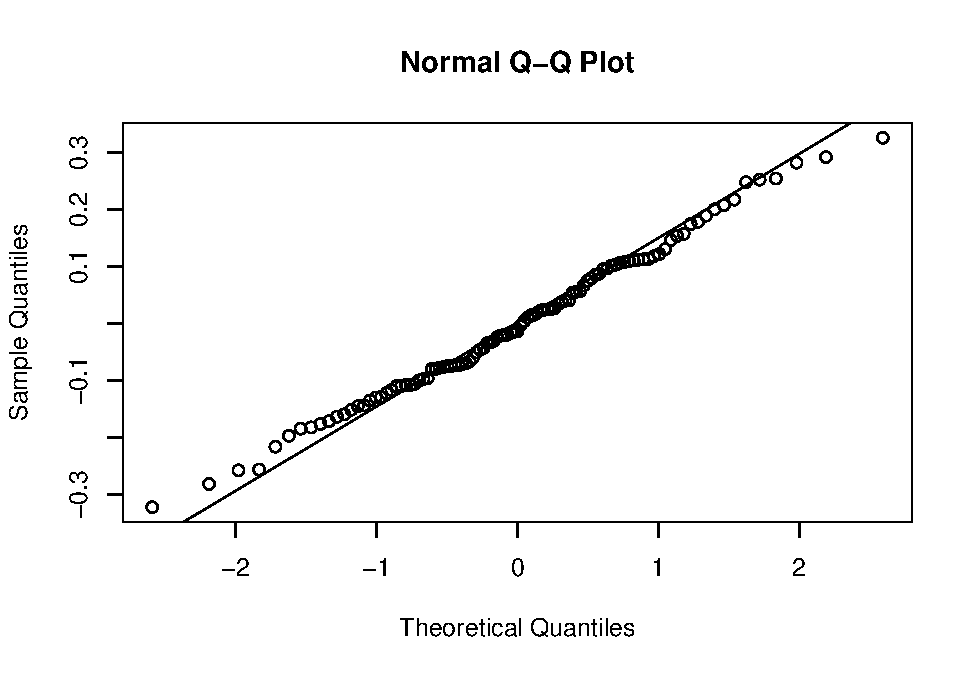
\includegraphics{code_files/figure-latex/unnamed-chunk-17-1.pdf}

\begin{Shaded}
\begin{Highlighting}[]
\CommentTok{\# H0: follows normality H1: does not follow normality}
\FunctionTok{shapiro.test}\NormalTok{(}\FunctionTok{resid}\NormalTok{(lmod\_all))}
\end{Highlighting}
\end{Shaded}

\begin{verbatim}
## 
##  Shapiro-Wilk normality test
## 
## data:  resid(lmod_all)
## W = 0.99248, p-value = 0.8337
\end{verbatim}

Tanto el test de Shapiro como el qqplot nos indican que los residuos
siguen una distribución normal. Podemos estar seguros porque aceptamos
la hipótesis nula del test (pv = 0.83) y en el gráfico los valores
siguen que manera bastante ajustada la recta.

\hypertarget{homocedasticidad}{%
\paragraph{Homocedasticidad}\label{homocedasticidad}}

\begin{Shaded}
\begin{Highlighting}[]
\CommentTok{\# Scale{-}Location plot}
\FunctionTok{plot}\NormalTok{(lmod\_all, }\AttributeTok{which =} \DecValTok{3}\NormalTok{)}
\end{Highlighting}
\end{Shaded}

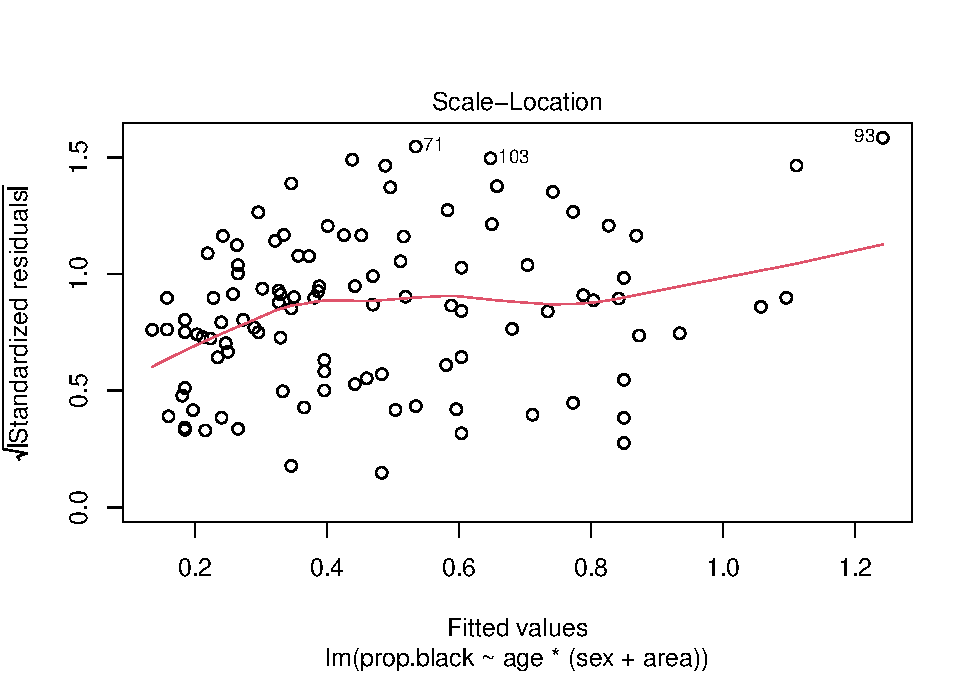
\includegraphics{code_files/figure-latex/unnamed-chunk-18-1.pdf}

\begin{Shaded}
\begin{Highlighting}[]
\CommentTok{\# Load required package}
\FunctionTok{library}\NormalTok{(lmtest)}
\end{Highlighting}
\end{Shaded}

\begin{verbatim}
## Loading required package: zoo
\end{verbatim}

\begin{verbatim}
## 
## Attaching package: 'zoo'
\end{verbatim}

\begin{verbatim}
## The following objects are masked from 'package:base':
## 
##     as.Date, as.Date.numeric
\end{verbatim}

\begin{verbatim}
## 
## Attaching package: 'lmtest'
\end{verbatim}

\begin{verbatim}
## The following object is masked from 'package:VGAM':
## 
##     lrtest
\end{verbatim}

\begin{Shaded}
\begin{Highlighting}[]
\CommentTok{\# Perform Breusch{-}Pagan test}
\FunctionTok{bptest}\NormalTok{(lmod\_all)}
\end{Highlighting}
\end{Shaded}

\begin{verbatim}
## 
##  studentized Breusch-Pagan test
## 
## data:  lmod_all
## BP = 10.316, df = 5, p-value = 0.06677
\end{verbatim}

\begin{Shaded}
\begin{Highlighting}[]
\FunctionTok{summary}\NormalTok{(}\FunctionTok{lm}\NormalTok{(}\FunctionTok{sqrt}\NormalTok{(}\FunctionTok{abs}\NormalTok{(}\FunctionTok{residuals}\NormalTok{(lmod\_all))) }\SpecialCharTok{\textasciitilde{}} \FunctionTok{fitted}\NormalTok{(lmod\_all)))}
\end{Highlighting}
\end{Shaded}

\begin{verbatim}
## 
## Call:
## lm(formula = sqrt(abs(residuals(lmod_all))) ~ fitted(lmod_all))
## 
## Residuals:
##       Min        1Q    Median        3Q       Max 
## -0.255173 -0.089350  0.003797  0.096214  0.256041 
## 
## Coefficients:
##                  Estimate Std. Error t value Pr(>|t|)    
## (Intercept)       0.25467    0.02478  10.276   <2e-16 ***
## fitted(lmod_all)  0.11205    0.04672   2.398   0.0183 *  
## ---
## Signif. codes:  0 '***' 0.001 '**' 0.01 '*' 0.05 '.' 0.1 ' ' 1
## 
## Residual standard error: 0.1181 on 103 degrees of freedom
## Multiple R-squared:  0.05289,    Adjusted R-squared:  0.04369 
## F-statistic: 5.752 on 1 and 103 DF,  p-value: 0.01827
\end{verbatim}

Parece ser que el modelo cumple homocedasticidad. En el gráfico podemos
ver como los valores tienen una forma bastante rectangular, y casi no
aumenta su dispersión a medida que aumenta el valor ajustado, aunque sí
lo hace ligeramente dando una ligera forma de cono.

De manera similar, el test de Breusch-Pagan nos indica que hay
homocedasticidad, ya que con pv = 0.06 aceptamos la hipótesis nula: la
varianza de los residuos es constante.

Por otro lado, en el resumen del modelo ajustado a la raíz cuadrada de
los residuos absolutos, observamos un pvalor significativo (pv = 0.01).
Esto sugiere que su relación no es aleatoria, y por lo tanto, el modelo
original viola homocedasticidad. Esta discrepancia puede deberse a
múltiples motivos, ya que el test de Breush-Pagan hace ciertas
asunciones como que los errores están normalmente distribuidos y tienen
varianza constante.

\hypertarget{independencia-de-errores}{%
\paragraph{Independencia de errores}\label{independencia-de-errores}}

\begin{Shaded}
\begin{Highlighting}[]
\CommentTok{\# Load the lmtest package}
\FunctionTok{library}\NormalTok{(lmtest)}

\CommentTok{\# Perform the Durbin{-}Watson test on lmod\_all}
\CommentTok{\#H0: No hay autocorrelación H1: Hay correlación}
\FunctionTok{dwtest}\NormalTok{(lmod\_all)}
\end{Highlighting}
\end{Shaded}

\begin{verbatim}
## 
##  Durbin-Watson test
## 
## data:  lmod_all
## DW = 0.83845, p-value = 5.739e-11
## alternative hypothesis: true autocorrelation is greater than 0
\end{verbatim}

\begin{Shaded}
\begin{Highlighting}[]
\CommentTok{\# Load the graphics package}
\FunctionTok{library}\NormalTok{(graphics)}

\CommentTok{\# Create a lag plot of the residuals from lmod\_all}
\FunctionTok{lag.plot}\NormalTok{(}\FunctionTok{resid}\NormalTok{(lmod\_all))}
\end{Highlighting}
\end{Shaded}

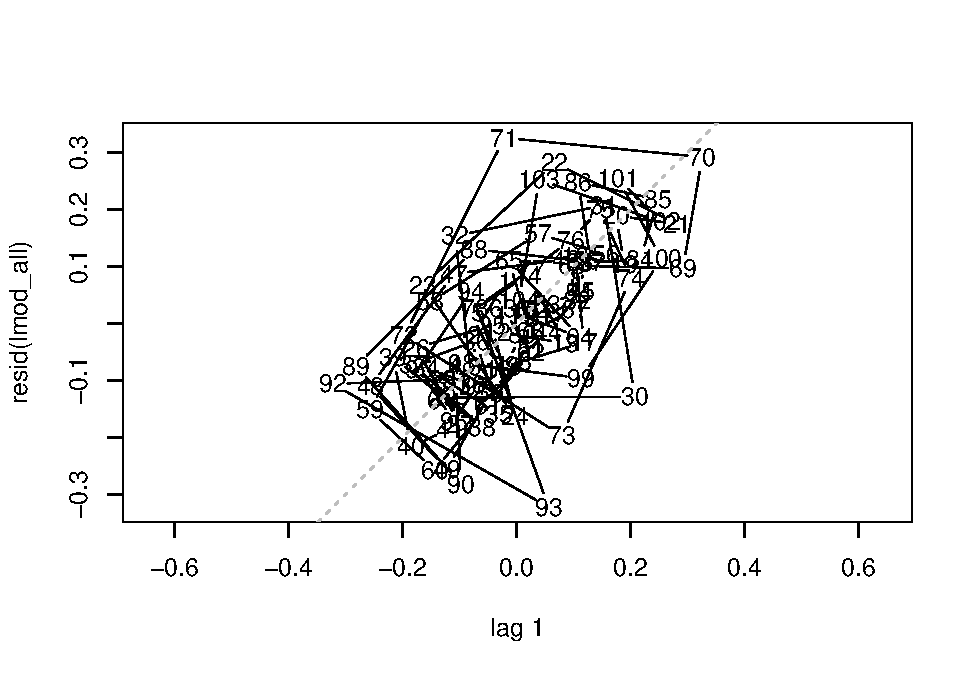
\includegraphics{code_files/figure-latex/unnamed-chunk-19-1.pdf}

Según el test de Durbin-Watson, hay evidencia de correlación de residuos
(pv \textless{} 0.05). Si miramos el gráfico, también determinados que
existe correlación de residuos, pues los puntos no se reparten
equitativamente sobre la línea horizontal y=0.

\hypertarget{correlaciuxf3n-de-variables}{%
\paragraph{Correlación de variables}\label{correlaciuxf3n-de-variables}}

\begin{Shaded}
\begin{Highlighting}[]
\FunctionTok{library}\NormalTok{(ggcorrplot)}

\CommentTok{\# Compute correlation matrix of independent variables}
\NormalTok{cor\_mat }\OtherTok{\textless{}{-}} \FunctionTok{cor}\NormalTok{(data2[, }\FunctionTok{c}\NormalTok{(}\StringTok{"age"}\NormalTok{, }\StringTok{"sexM"}\NormalTok{, }\StringTok{"areaS"}\NormalTok{)])}

\CommentTok{\# Create correlation plot}
\FunctionTok{ggcorrplot}\NormalTok{(cor\_mat, }\AttributeTok{hc.order =} \ConstantTok{TRUE}\NormalTok{, }\AttributeTok{type =} \StringTok{"lower"}\NormalTok{, }\AttributeTok{lab =} \ConstantTok{TRUE}\NormalTok{)}
\end{Highlighting}
\end{Shaded}

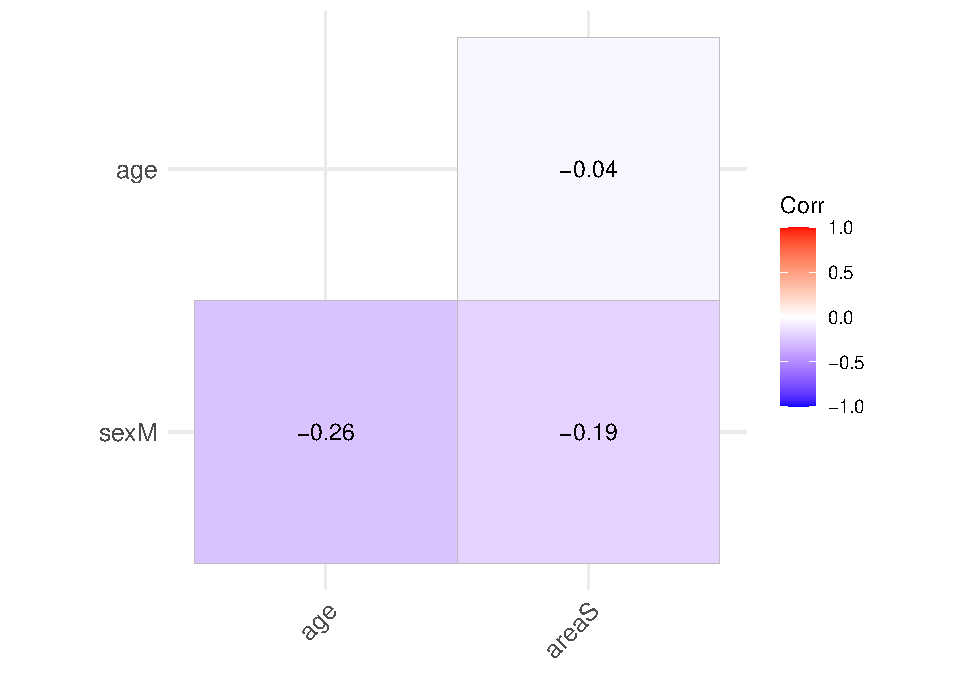
\includegraphics{code_files/figure-latex/unnamed-chunk-20-1.pdf}

\begin{Shaded}
\begin{Highlighting}[]
\CommentTok{\# Compute correlation and p{-}value between age and dummy\_sex}
\FunctionTok{cor.test}\NormalTok{(data2}\SpecialCharTok{$}\NormalTok{age, data2}\SpecialCharTok{$}\NormalTok{sexM)}
\end{Highlighting}
\end{Shaded}

\begin{verbatim}
## 
##  Pearson's product-moment correlation
## 
## data:  data2$age and data2$sexM
## t = -2.7308, df = 103, p-value = 0.007434
## alternative hypothesis: true correlation is not equal to 0
## 95 percent confidence interval:
##  -0.43007820 -0.07173848
## sample estimates:
##        cor 
## -0.2598311
\end{verbatim}

\begin{Shaded}
\begin{Highlighting}[]
\CommentTok{\# Compute correlation and p{-}value between age and dummy\_area}
\FunctionTok{cor.test}\NormalTok{(data2}\SpecialCharTok{$}\NormalTok{age, data2}\SpecialCharTok{$}\NormalTok{areaS)}
\end{Highlighting}
\end{Shaded}

\begin{verbatim}
## 
##  Pearson's product-moment correlation
## 
## data:  data2$age and data2$areaS
## t = -0.45041, df = 103, p-value = 0.6534
## alternative hypothesis: true correlation is not equal to 0
## 95 percent confidence interval:
##  -0.2340136  0.1485910
## sample estimates:
##         cor 
## -0.04433691
\end{verbatim}

\begin{Shaded}
\begin{Highlighting}[]
\CommentTok{\# Compute correlation and p{-}value between dummy\_sex and dummy\_area}
\FunctionTok{cor.test}\NormalTok{(data2}\SpecialCharTok{$}\NormalTok{areaS, data2}\SpecialCharTok{$}\NormalTok{sexM)}
\end{Highlighting}
\end{Shaded}

\begin{verbatim}
## 
##  Pearson's product-moment correlation
## 
## data:  data2$areaS and data2$sexM
## t = -1.9235, df = 103, p-value = 0.05718
## alternative hypothesis: true correlation is not equal to 0
## 95 percent confidence interval:
##  -0.364854816  0.005655778
## sample estimates:
##        cor 
## -0.1862113
\end{verbatim}

Existe correlación entre las variables sexo y edad. Parece ser que los
machos tienen menor edad que las hembras (-0.26), y esta relación es
significativa (pv = 0.007). El resto de variables no parecen estar
correlacionadas.

\hypertarget{media-condicional-de-0}{%
\paragraph{Media condicional de 0}\label{media-condicional-de-0}}

\begin{Shaded}
\begin{Highlighting}[]
\CommentTok{\# H0: Intercept pv = 0 H1: Distinto de 0}
\FunctionTok{summary}\NormalTok{(lmod\_all)}
\end{Highlighting}
\end{Shaded}

\begin{verbatim}
## 
## Call:
## lm(formula = prop.black ~ age * (sex + area), data = data2)
## 
## Residuals:
##      Min       1Q   Median       3Q      Max 
## -0.32206 -0.09746 -0.01365  0.10173  0.32558 
## 
## Coefficients:
##              Estimate Std. Error t value Pr(>|t|)    
## (Intercept)  0.003101   0.105559   0.029 0.976627    
## age          0.081609   0.021302   3.831 0.000224 ***
## sexM        -0.005786   0.071180  -0.081 0.935374    
## areaS        0.069820   0.106242   0.657 0.512593    
## age:sexM    -0.015094   0.017246  -0.875 0.383571    
## age:areaS   -0.004692   0.021184  -0.221 0.825161    
## ---
## Signif. codes:  0 '***' 0.001 '**' 0.01 '*' 0.05 '.' 0.1 ' ' 1
## 
## Residual standard error: 0.1373 on 99 degrees of freedom
## Multiple R-squared:  0.7738, Adjusted R-squared:  0.7624 
## F-statistic: 67.74 on 5 and 99 DF,  p-value: < 2.2e-16
\end{verbatim}

Podemos ver que el pvalor del intercepto no es significativo, y por
tanto aceptamos la hipótesis nula de que la media condicional de los
errores es 0. Es importante que la media condicional sea 0, ya que si no
el modelo sobreestimaría o subestimaría los valores reales de la
población, llevando así a predicciones sesgadas.

\hypertarget{observaciones-inusuales}{%
\paragraph{Observaciones inusuales}\label{observaciones-inusuales}}

\begin{Shaded}
\begin{Highlighting}[]
\CommentTok{\# Leverage}

\CommentTok{\# Calculate the threshold based on the rule of thumb}
\NormalTok{p }\OtherTok{\textless{}{-}} \FunctionTok{ncol}\NormalTok{(}\FunctionTok{model.matrix}\NormalTok{(lmod\_all)) }\SpecialCharTok{{-}} \DecValTok{1}
\NormalTok{n }\OtherTok{\textless{}{-}} \FunctionTok{nrow}\NormalTok{(data2)}
\NormalTok{threshold }\OtherTok{\textless{}{-}} \DecValTok{2}\SpecialCharTok{*}\NormalTok{p}\SpecialCharTok{/}\NormalTok{n}

\CommentTok{\# Calculate the number of observations with hat values above the threshold}
\NormalTok{hatv }\OtherTok{\textless{}{-}} \FunctionTok{hatvalues}\NormalTok{(lmod\_all)}
\NormalTok{num\_outliers }\OtherTok{\textless{}{-}} \FunctionTok{sum}\NormalTok{(hatv }\SpecialCharTok{\textgreater{}}\NormalTok{ threshold)}

\CommentTok{\# Print the number of outliers}
\FunctionTok{cat}\NormalTok{(}\StringTok{"Number of outliers according to hatvalues:"}\NormalTok{, num\_outliers)}
\end{Highlighting}
\end{Shaded}

\begin{verbatim}
## Number of outliers according to hatvalues: 11
\end{verbatim}

\begin{Shaded}
\begin{Highlighting}[]
\CommentTok{\# Half normal plot with hatvalues}
\FunctionTok{library}\NormalTok{(faraway)}
\end{Highlighting}
\end{Shaded}

\begin{verbatim}
## 
## Attaching package: 'faraway'
\end{verbatim}

\begin{verbatim}
## The following object is masked from 'package:rpart':
## 
##     solder
\end{verbatim}

\begin{verbatim}
## The following objects are masked from 'package:VGAM':
## 
##     hormone, logit, pneumo, prplot
\end{verbatim}

\begin{verbatim}
## The following objects are masked from 'package:car':
## 
##     logit, vif
\end{verbatim}

\begin{Shaded}
\begin{Highlighting}[]
\FunctionTok{halfnorm}\NormalTok{(hatv, }\AttributeTok{ylab=}\StringTok{"Hatvalues"}\NormalTok{)}
\end{Highlighting}
\end{Shaded}

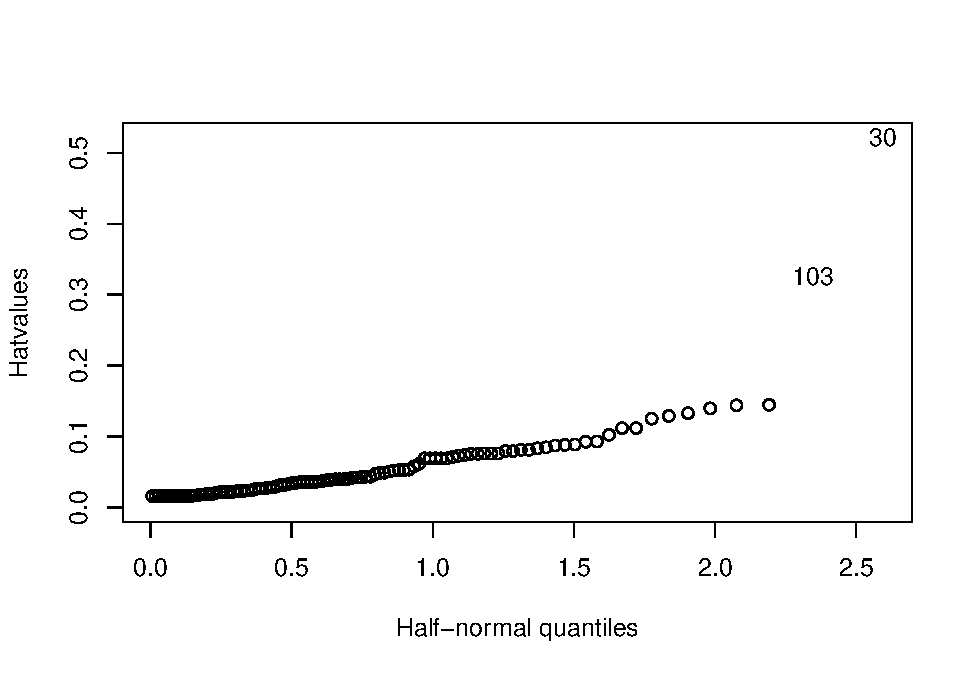
\includegraphics{code_files/figure-latex/unnamed-chunk-22-1.pdf}

\begin{Shaded}
\begin{Highlighting}[]
\CommentTok{\# Half normal plot with cook\textquotesingle{}s distance}
\NormalTok{cook }\OtherTok{=} \FunctionTok{cooks.distance}\NormalTok{(lmod\_all)}
\FunctionTok{halfnorm}\NormalTok{(cook, }\AttributeTok{ylab=}\StringTok{"Cook\textquotesingle{}s distances"}\NormalTok{)}
\end{Highlighting}
\end{Shaded}

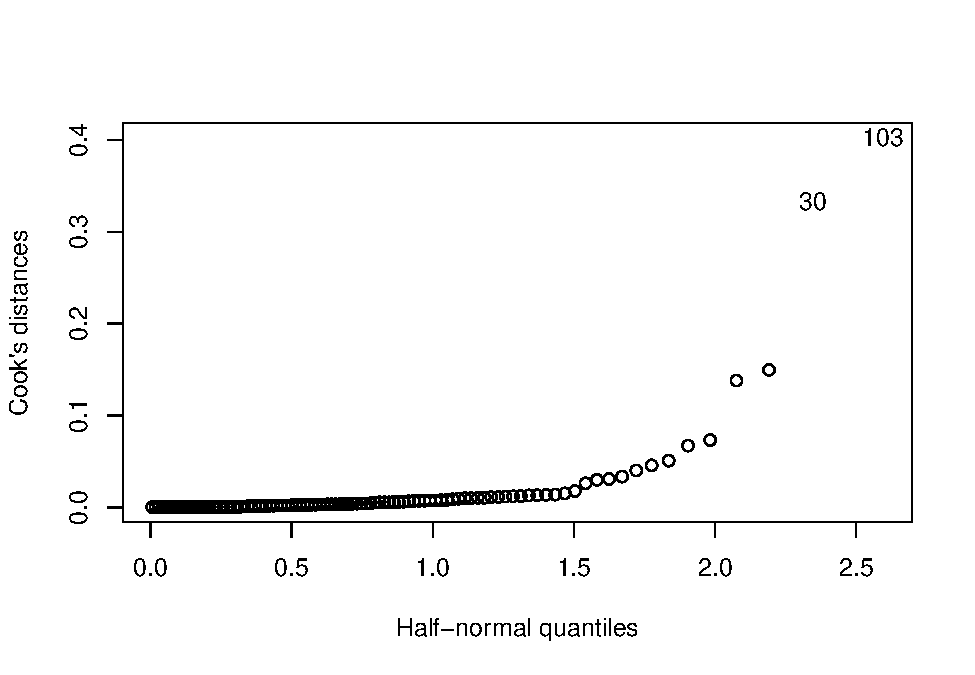
\includegraphics{code_files/figure-latex/unnamed-chunk-22-2.pdf}

En estadística, un punto influyente es un punto que tiene un gran efecto
en la estimación de los coeficientes de regresión de un modelo. Vemos
que en este estudio existen múltiples puntos influyentes con valores
atípicos de las variables dependientes (90, 93, 30\ldots). Si usamos la
regla general de 2p/n (siendo p el número de variables independientes
del modelo y n el tamaño muestral), obtenemos 11 puntos influyentes.
Mirando el gráfico Half-normal de hatvalues, podemos ver que
efectivamente son aproximadamente 11 los puntos que se desvían de la
recta principal.

Por otro lado, calculamos la distancia de cook para cada uno de los
puntos. Mientras que el hatvalue mide cuán desviado está un punto del
centro de los datos en cuanto a variables dependientes, la distancia de
cook mide el efecto que tendría eliminar el punto en el modelo. En este
nuevo gráfico, parece son 13 los puntos más influyentes.

\begin{Shaded}
\begin{Highlighting}[]
\CommentTok{\# Outliers}

\NormalTok{stud }\OtherTok{=} \FunctionTok{rstudent}\NormalTok{(lmod\_all)}
\NormalTok{maxo }\OtherTok{=}\NormalTok{ stud[}\FunctionTok{which.max}\NormalTok{(}\FunctionTok{abs}\NormalTok{(stud))]}
\CommentTok{\# Calculate Bonferroni critical value}
\NormalTok{bonf\_crit }\OtherTok{\textless{}{-}} \FunctionTok{qt}\NormalTok{(}\FloatTok{0.05}\SpecialCharTok{/}\NormalTok{(}\DecValTok{2}\SpecialCharTok{*}\NormalTok{n), }\AttributeTok{df =}\NormalTok{ lmod\_all}\SpecialCharTok{$}\NormalTok{df.residual)}

\FunctionTok{cat}\NormalTok{(}\StringTok{"}\SpecialCharTok{\textbackslash{}n}\StringTok{"}\NormalTok{)}
\end{Highlighting}
\end{Shaded}

\begin{Shaded}
\begin{Highlighting}[]
\ControlFlowTok{if}\NormalTok{ (maxo }\SpecialCharTok{\textgreater{}} \FunctionTok{abs}\NormalTok{(bonf\_crit)) \{}
  \FunctionTok{cat}\NormalTok{(}\StringTok{"The point is an outlier"}\NormalTok{)}
\NormalTok{\} }\ControlFlowTok{else}\NormalTok{ \{}
  \FunctionTok{cat}\NormalTok{(}\StringTok{"The point is not an outlier"}\NormalTok{)}
\NormalTok{\}}
\end{Highlighting}
\end{Shaded}

\begin{verbatim}
## The point is not an outlier
\end{verbatim}

En estadística, un outlier es un punto significativamente distinto al
resto. En este estudio parece que no tenemos outliers. Un punto
influyente no tiene porque ser un outlier y un outlier no tiene porque
ser un punto influyente. En el artículo original contaban con algún
outlier que fue eliminado, como nuestros datos están extrapolados del
artículo no contienen outliers.

\hypertarget{conclusiuxf3n}{%
\paragraph{Conclusión}\label{conclusiuxf3n}}

A pesar que nuestro modelo cumple con muchas de las características, no
podemos afirmar que sea un buen modelo. El motivo principal es la falta
de linealidad. No podemos ajustar un buen modelo lineal a variables que
no tienen una relación lineal. Sería adecuado realizar algún tipo de
transformación para poder ajustar un modelo lineal, o bien ajustar un
modelo no-lineal.

Cabe destacar que a pesar que el modelo no cumpla todas las asunciones,
no significa que no nos proporcione información útil y buenas
predicciones, pero es extremadamente importante interpretar los
resultados con cautela y tener en mente las limitaciones del modelo.

\hypertarget{b-variable-respuesta-proporciuxf3n}{%
\subsubsection{(b) Variable respuesta
proporción}\label{b-variable-respuesta-proporciuxf3n}}

El mayor problema que conlleva el hecho de que la variable dependiente
sea una proporción, es que nuestro modelo podría predecir valores que no
son posibles (por debajo de 0 o encima de 1). Adicionalmente, las
relaciones de estas proporciones no siguen una linea recta, si no una
sigmoidal (con forma de ``S''). Es común también que este tipo de
modelos con proporciones no presenten homocedasticidad y normalidad de
errores.

Para mejorar el ajuste de los datos existen múltiples opciones. Se puede
realizar una regresión beta o regresión de respuesta fraccional. En la
regresión beta los valores predichos se encuentran entre 0 y 1 (no
incluidos).

Otra aproximación que se puede realizar, es una transformación de los
datos. Se pueden realizar ciertas transformaciones (como hacer la raíz
cuadrada), para que los datos se alejen de los extremos (0 y 1). Con
valores entre 0.2 y 0.8 nuestro modelo no debería llegar a predecir
valores fuera del rango entre 0 y 1.

En este caso en particular, se puede aplicar esta transformación
aplicando la raíz cuadrada. Por otro lado, se podría medir la cantidad
de negro en la nariz de los leones por milímetro cuadrado, y así esta
variable dejaría de ser una proporción y no presentaría estos problemas.

\hypertarget{c-transformaciuxf3n-de-la-variable-dependiente}{%
\subsubsection{(c) Transformación de la variable
dependiente}\label{c-transformaciuxf3n-de-la-variable-dependiente}}

Dado que la variable respuesta es una proporción, y no acaba de
ajustarse a una relación lineal, realizaremos una transformación
arcsin(sqrt) a la variable respuesta. He escogido esta transformación
antes que la logit, porque la transformación logit se suele usar en
casos donde la proporción representa un resultado binario (ej:
proporción de leones con nariz negra). Mientras que arcsin se suele usar
para representar una variable continua (ej: proporción negra de la
nariz).

\begin{Shaded}
\begin{Highlighting}[]
\CommentTok{\# Comprobamos que los datos están entre 0 y 1, si no no podemos aplicar la transformación}
\FunctionTok{min}\NormalTok{(data2}\SpecialCharTok{$}\NormalTok{prop.black)}
\end{Highlighting}
\end{Shaded}

\begin{verbatim}
## [1] 0.05
\end{verbatim}

\begin{Shaded}
\begin{Highlighting}[]
\FunctionTok{max}\NormalTok{(data2}\SpecialCharTok{$}\NormalTok{prop.black)}
\end{Highlighting}
\end{Shaded}

\begin{verbatim}
## [1] 0.99
\end{verbatim}

\begin{Shaded}
\begin{Highlighting}[]
\CommentTok{\# Aplicamos la transformación}
\NormalTok{prop.black.transformed }\OtherTok{=} \FunctionTok{asin}\NormalTok{(}\FunctionTok{sqrt}\NormalTok{(data2}\SpecialCharTok{$}\NormalTok{prop.black))}
\CommentTok{\# Rehacemos el modelo}
\NormalTok{lmod\_all\_transformed }\OtherTok{=} \FunctionTok{lm}\NormalTok{(prop.black.transformed }\SpecialCharTok{\textasciitilde{}}\NormalTok{ age }\SpecialCharTok{*}\NormalTok{ (sex }\SpecialCharTok{+}\NormalTok{ area), }\AttributeTok{data =}\NormalTok{ data2)}

\FunctionTok{summary}\NormalTok{(lmod\_all\_transformed)}
\end{Highlighting}
\end{Shaded}

\begin{verbatim}
## 
## Call:
## lm(formula = prop.black.transformed ~ age * (sex + area), data = data2)
## 
## Residuals:
##      Min       1Q   Median       3Q      Max 
## -0.37787 -0.10177 -0.01389  0.10657  0.39591 
## 
## Coefficients:
##              Estimate Std. Error t value Pr(>|t|)    
## (Intercept)  0.220586   0.122869   1.795 0.075657 .  
## age          0.094754   0.024796   3.821 0.000232 ***
## sexM         0.023239   0.082852   0.280 0.779691    
## areaS        0.068191   0.123663   0.551 0.582588    
## age:sexM    -0.023067   0.020074  -1.149 0.253298    
## age:areaS   -0.004416   0.024657  -0.179 0.858234    
## ---
## Signif. codes:  0 '***' 0.001 '**' 0.01 '*' 0.05 '.' 0.1 ' ' 1
## 
## Residual standard error: 0.1598 on 99 degrees of freedom
## Multiple R-squared:  0.7716, Adjusted R-squared:   0.76 
## F-statistic: 66.87 on 5 and 99 DF,  p-value: < 2.2e-16
\end{verbatim}

\begin{Shaded}
\begin{Highlighting}[]
\FunctionTok{library}\NormalTok{(knitr)}

\CommentTok{\# Calculate the goodness{-}of{-}fit metrics}
\FunctionTok{library}\NormalTok{(broom) }\CommentTok{\# Usaremos la función augment para calcular los residuos (diferencia entre valores predichos y valores observados)}

\NormalTok{R }\OtherTok{=} \FunctionTok{summary}\NormalTok{(lmod\_all)}\SpecialCharTok{$}\NormalTok{r.squared}
\NormalTok{Rad }\OtherTok{=} \FunctionTok{summary}\NormalTok{(lmod\_all)}\SpecialCharTok{$}\NormalTok{adj.r.squared}
\NormalTok{rmse }\OtherTok{=} \FunctionTok{sqrt}\NormalTok{(}\FunctionTok{mean}\NormalTok{(}\FunctionTok{augment}\NormalTok{(lmod\_all)}\SpecialCharTok{$}\NormalTok{.resid}\SpecialCharTok{\^{}}\DecValTok{2}\NormalTok{))}
\NormalTok{aic }\OtherTok{=} \FunctionTok{AIC}\NormalTok{(lmod\_all)}
\NormalTok{R\_t }\OtherTok{=} \FunctionTok{summary}\NormalTok{(lmod\_all\_transformed)}\SpecialCharTok{$}\NormalTok{r.squared}
\NormalTok{Rad\_t }\OtherTok{=} \FunctionTok{summary}\NormalTok{(lmod\_all\_transformed)}\SpecialCharTok{$}\NormalTok{adj.r.squared}
\NormalTok{rmse\_t }\OtherTok{=} \FunctionTok{sqrt}\NormalTok{(}\FunctionTok{mean}\NormalTok{(}\FunctionTok{augment}\NormalTok{(lmod\_all\_transformed)}\SpecialCharTok{$}\NormalTok{.resid}\SpecialCharTok{\^{}}\DecValTok{2}\NormalTok{))}
\NormalTok{aic\_t }\OtherTok{=} \FunctionTok{AIC}\NormalTok{(lmod\_all\_transformed)}

\CommentTok{\# Create table}
\NormalTok{metrics\_df }\OtherTok{\textless{}{-}} \FunctionTok{bind\_rows}\NormalTok{(}
    \FunctionTok{augment}\NormalTok{(lmod\_all) }\SpecialCharTok{\%\textgreater{}\%} \FunctionTok{summarise}\NormalTok{(}\AttributeTok{Modelo =} \StringTok{"Sin transformar"}\NormalTok{, }\AttributeTok{R\_squared =}\NormalTok{ R, }\AttributeTok{Adj\_R\_squared =}\NormalTok{ Rad, }\AttributeTok{rmse =}\NormalTok{ rmse, }\AttributeTok{AIC =}\NormalTok{ aic),}
    \FunctionTok{augment}\NormalTok{(lmod\_all\_transformed) }\SpecialCharTok{\%\textgreater{}\%} \FunctionTok{summarise}\NormalTok{(}\AttributeTok{Modelo =} \StringTok{"Arcsin(sqrt)"}\NormalTok{, }\AttributeTok{R\_squared =}\NormalTok{ R\_t, }\AttributeTok{Adj\_R\_squared =}\NormalTok{ Rad\_t, }\AttributeTok{rmse =}\NormalTok{ rmse\_t, }\AttributeTok{AIC =}\NormalTok{ aic\_t)}
\NormalTok{)}

\CommentTok{\# Print the table}
\FunctionTok{kable}\NormalTok{(metrics\_df, }\AttributeTok{format =} \StringTok{"markdown"}\NormalTok{)}
\end{Highlighting}
\end{Shaded}

\begin{longtable}[]{@{}lrrrr@{}}
\toprule()
Modelo & R\_squared & Adj\_R\_squared & rmse & AIC \\
\midrule()
\endhead
Sin transformar & 0.7738200 & 0.7623968 & 0.1333169 & -111.17838 \\
Arcsin(sqrt) & 0.7715525 & 0.7600147 & 0.1551784 & -79.29063 \\
\bottomrule()
\end{longtable}

En cuanto a significación del modelo no vemos ninguna diferencia. Ambos
cuentan con un pvalor significativo. En cuanto a la R, ésta indica el
porcentaje de variabilidad de la varianle dependiente que es explicado
por el modelo. En ambos casos es 0.77, este resultado implica que
aproximadamente un 77\% de la proporción de negro en las narices de los
leones es explicada por las variables y modelo usado. Es un poco pobre,
ya que hay un 23\% de variabilidad que no podemos explicar.

El rmse o error cuadrático medio calcula la cantidad de error entre los
valores predichos por el modelo y los valores reales observados. Por lo
tanto, cuanto menor sea este error, mejor predice nuestro modelo los
datos usados. En este caso, parece que el modelo sin transformar predice
ligeramente mejor los datos.

El AIC es una medida de la calidad relativa del modelo. Permite comparar
modelos teniendo en cuenta su complejidad. Nuevamente, valores menores
de AIC indican mejor ajuste, de manera que el modelo sin transformar se
ajusta mejor a los datos que el transformado.

Tras estudiar estos parámetros, concluimos que el modelo sin transformar
es mejor, puesto que es el más sencillo y se ajusta igual de bien o
mejor que el modelo transformado.

\hypertarget{d-diagnuxf3stico-ruxe1pido}{%
\subsubsection{(d) Diagnóstico
rápido}\label{d-diagnuxf3stico-ruxe1pido}}

Puesto que nuestra principal preocupación era la no-relación lineal
entre las variables independientes y la dependiente, vale la pena
estudiar si ésta ha mejorado.

\begin{Shaded}
\begin{Highlighting}[]
\CommentTok{\# Load required packages}
\FunctionTok{library}\NormalTok{(ggplot2)}

\CommentTok{\# Residuals vs. Fitted plot}
\FunctionTok{plot}\NormalTok{(lmod\_all\_transformed, }\AttributeTok{which =} \DecValTok{1}\NormalTok{)}
\end{Highlighting}
\end{Shaded}

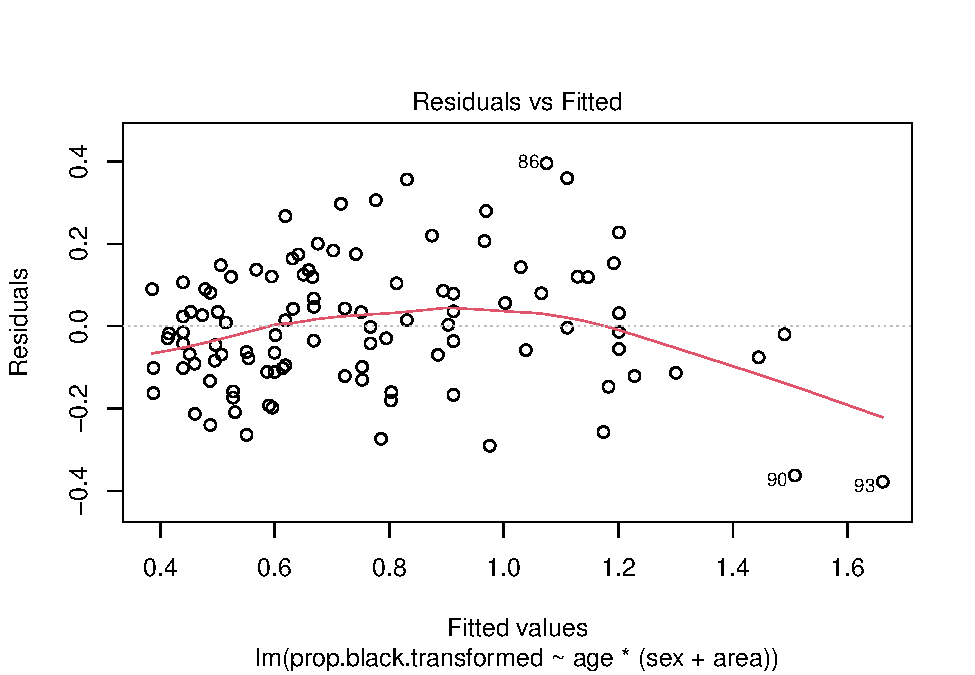
\includegraphics{code_files/figure-latex/unnamed-chunk-25-1.pdf}

\begin{Shaded}
\begin{Highlighting}[]
\CommentTok{\# Add quadratic terms for age, sex, and area to lmod\_all}
\NormalTok{lmod\_quad\_transformed }\OtherTok{=} \FunctionTok{lm}\NormalTok{(prop.black.transformed }\SpecialCharTok{\textasciitilde{}}\NormalTok{ age }\SpecialCharTok{*}\NormalTok{ (dummy\_sex }\SpecialCharTok{+}\NormalTok{ dummy\_area) }\SpecialCharTok{+} \FunctionTok{I}\NormalTok{(age}\SpecialCharTok{\^{}}\DecValTok{2}\NormalTok{) }\SpecialCharTok{*}\NormalTok{ (}\FunctionTok{I}\NormalTok{(dummy\_sex}\SpecialCharTok{\^{}}\DecValTok{2}\NormalTok{) }\SpecialCharTok{+} \FunctionTok{I}\NormalTok{(dummy\_area}\SpecialCharTok{\^{}}\DecValTok{2}\NormalTok{)), }\AttributeTok{data =}\NormalTok{ data2)}

\CommentTok{\# Perform an F{-}test to compare lmod\_all and lmod\_quad}
\FunctionTok{anova}\NormalTok{(lmod\_all\_transformed, lmod\_quad\_transformed)}
\end{Highlighting}
\end{Shaded}

\begin{verbatim}
## Analysis of Variance Table
## 
## Model 1: prop.black.transformed ~ age * (sex + area)
## Model 2: prop.black.transformed ~ age * (dummy_sex + dummy_area) + I(age^2) * 
##     (I(dummy_sex^2) + I(dummy_area^2))
##   Res.Df    RSS Df Sum of Sq      F    Pr(>F)    
## 1     99 2.5284                                  
## 2     96 2.0914  3   0.43703 6.6869 0.0003795 ***
## ---
## Signif. codes:  0 '***' 0.001 '**' 0.01 '*' 0.05 '.' 0.1 ' ' 1
\end{verbatim}

\begin{Shaded}
\begin{Highlighting}[]
\CommentTok{\# Normalidad}
\CommentTok{\# Normality of residuals}
\FunctionTok{qqnorm}\NormalTok{(}\FunctionTok{resid}\NormalTok{(lmod\_all\_transformed))}
\FunctionTok{qqline}\NormalTok{(}\FunctionTok{resid}\NormalTok{(lmod\_all\_transformed))}
\end{Highlighting}
\end{Shaded}

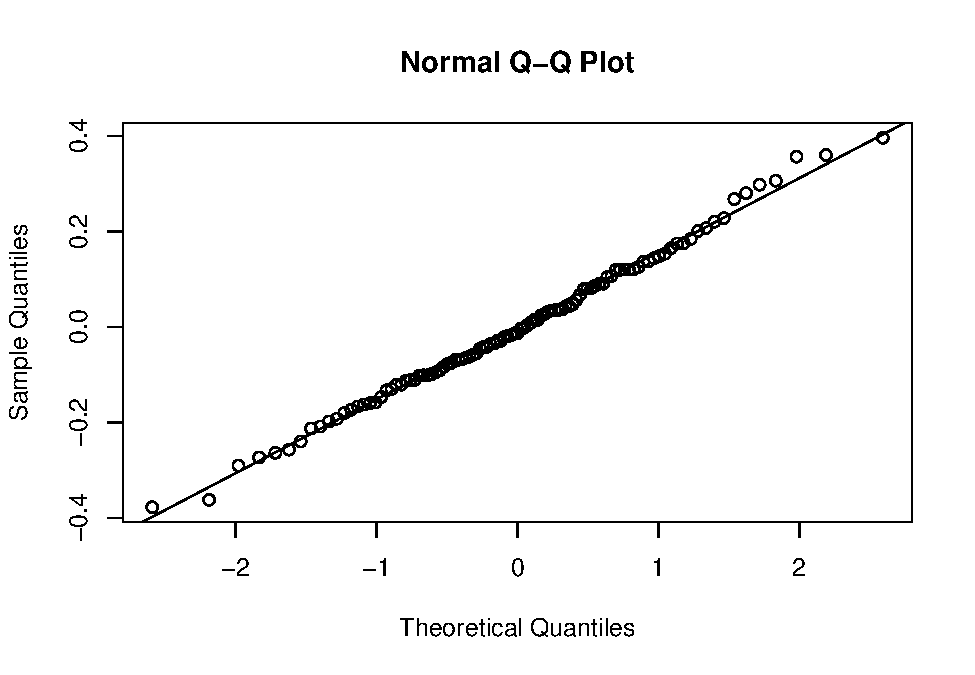
\includegraphics{code_files/figure-latex/unnamed-chunk-25-2.pdf}

\begin{Shaded}
\begin{Highlighting}[]
\CommentTok{\# H0: follows normality H1: does not follow normality}
\FunctionTok{shapiro.test}\NormalTok{(}\FunctionTok{resid}\NormalTok{(lmod\_all\_transformed))}
\end{Highlighting}
\end{Shaded}

\begin{verbatim}
## 
##  Shapiro-Wilk normality test
## 
## data:  resid(lmod_all_transformed)
## W = 0.99408, p-value = 0.9332
\end{verbatim}

\begin{Shaded}
\begin{Highlighting}[]
\CommentTok{\# Homocedasticidad}
\CommentTok{\# Scale{-}Location plot}
\FunctionTok{plot}\NormalTok{(lmod\_all\_transformed, }\AttributeTok{which =} \DecValTok{3}\NormalTok{)}
\end{Highlighting}
\end{Shaded}

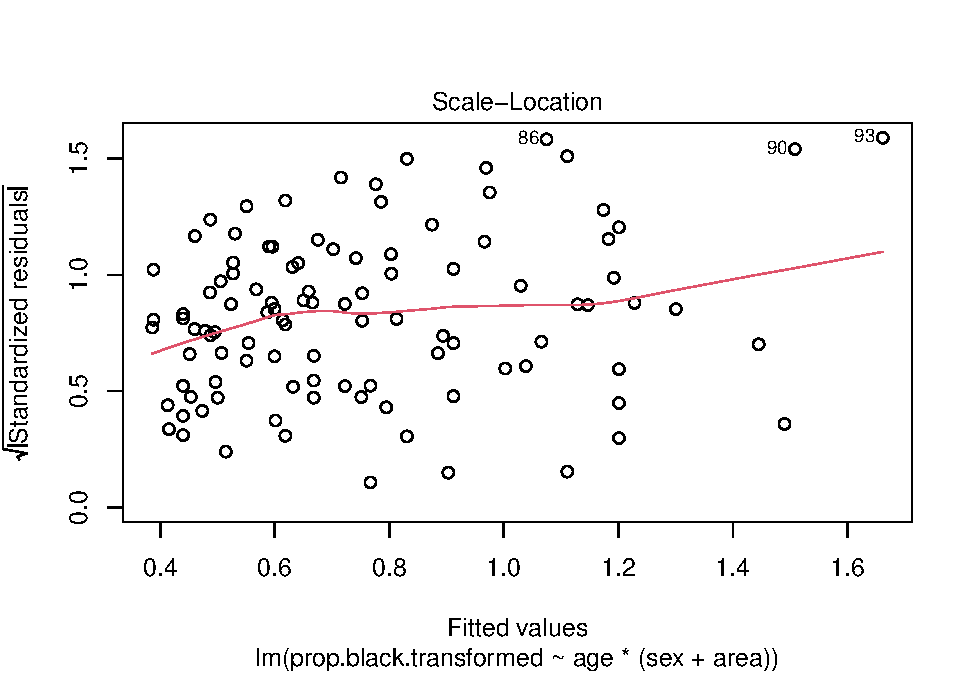
\includegraphics{code_files/figure-latex/unnamed-chunk-25-3.pdf}

\begin{Shaded}
\begin{Highlighting}[]
\CommentTok{\# Load required package}
\FunctionTok{library}\NormalTok{(lmtest)}
\CommentTok{\# Perform Breusch{-}Pagan test}
\FunctionTok{bptest}\NormalTok{(lmod\_all\_transformed)}
\end{Highlighting}
\end{Shaded}

\begin{verbatim}
## 
##  studentized Breusch-Pagan test
## 
## data:  lmod_all_transformed
## BP = 11.571, df = 5, p-value = 0.04117
\end{verbatim}

\begin{Shaded}
\begin{Highlighting}[]
\FunctionTok{summary}\NormalTok{(}\FunctionTok{lm}\NormalTok{(}\FunctionTok{sqrt}\NormalTok{(}\FunctionTok{abs}\NormalTok{(}\FunctionTok{residuals}\NormalTok{(lmod\_all\_transformed))) }\SpecialCharTok{\textasciitilde{}} \FunctionTok{fitted}\NormalTok{(lmod\_all\_transformed)))}
\end{Highlighting}
\end{Shaded}

\begin{verbatim}
## 
## Call:
## lm(formula = sqrt(abs(residuals(lmod_all_transformed))) ~ fitted(lmod_all_transformed))
## 
## Residuals:
##       Min        1Q    Median        3Q       Max 
## -0.295560 -0.109175  0.004272  0.096188  0.276074 
## 
## Coefficients:
##                              Estimate Std. Error t value Pr(>|t|)    
## (Intercept)                   0.25610    0.03727   6.871    5e-10 ***
## fitted(lmod_all_transformed)  0.09030    0.04601   1.963   0.0524 .  
## ---
## Signif. codes:  0 '***' 0.001 '**' 0.01 '*' 0.05 '.' 0.1 ' ' 1
## 
## Residual standard error: 0.1344 on 103 degrees of freedom
## Multiple R-squared:  0.03605,    Adjusted R-squared:  0.02669 
## F-statistic: 3.852 on 1 and 103 DF,  p-value: 0.05239
\end{verbatim}

Parece ser que no ha mejorado la linealidad a pesar de la
transformación. Sí ha mejorado la normalidad (como podemos ver en el
QQ-plot, ya que se ajusta mejor a la línea recta), aunque en el modelo
sin transformar ya se seguía normalidad. En cuanto a la
homocedasticidad, aunque ahora el test de Breusch-Pagan indica
heterocedasticidad, en el modelo de regresión sobre los residuos podemos
ver que sí ha mejorado la heterocedasticidad, ya que ahora el pvalor no
es significativo.

A pesar de las mejoras en normalidad y homocedasticidad, seguimos
insatisfechos con el modelo ajustado, ya que sigue sin cumplir
linealidad.

Por otro lado, la adición de interacciones o variables podría ayudar el
ajuste del modelo, pero también aportaría complejidad y dificultad a la
hora de analizar los resultados. Realizar un pre-procesamiento adicional
de los datos también sería posible, como una estandarización o una
transformación distinta de la variable dependiente, ya que arcsin(sqrt)
no ha funcionado. Si esto falla, deberíamos considerar usar otro tipo de
regresión. Si la relación entre las variables independientes y la
variable dependiente no es lineal, debemos considerar realizar otro tipo
de regresión como la logística.

\hypertarget{e-discusiuxf3n-uso-arcsin}{%
\subsubsection{(e) Discusión uso
arcsin}\label{e-discusiuxf3n-uso-arcsin}}

Tal y como comentamos en el apartado 2d, el modelo que proponen en el
artículo utiliza la función arcsin(sqrt) para transformar la proporción
de negro en la nariz, y hacerla más simétrica y adecuada para el estudio
estadístico. Con esta transformación, los valores medios de proporción
(0.3-0.7) siguen una distribución normal, gracias a esto se puede
realizar una regresión lineal.

Se define de la siguiente manera: arcsin(sqrt(x)) =
sin\^{}(-1)(\(\sqrt{x}\)). La transformación sqrt estabiliza la
varianza, haciendo que los valores más extremos (cercanos a 0 y 1), se
desplacen hacia el centro, ayudando así a que caigan en la zona de
máxima linealidad.

\includegraphics[width=0.6\textwidth,height=\textheight]{C:/Users/Arialux/Documents/ShareX/Screenshots/2023-05/firefox_YHMpOEbHLE.png}

\hypertarget{anexo}{%
\section{ANEXO}\label{anexo}}

\end{document}
